\documentclass[12pt,a4paper]{report}

% Page Geometry (Left: 1.25in, Right: 1.0in, Top: 1.0in, Bottom: 1.0in)
\usepackage[left=1.25in,right=1.0in,top=1.0in,bottom=1.0in]{geometry}

% Typography & Spacing
\usepackage{times}
\usepackage{setspace}
\setstretch{1.3}
\usepackage{microtype}

% Mathematical Formatting
\usepackage{amsmath,amssymb,amsfonts}

% Graphics & Tables
\usepackage{graphicx}
\usepackage{booktabs}
\usepackage{tabularx}
\usepackage{array}
\usepackage{caption}
\usepackage{subcaption}

% Headers and Footers
\usepackage{fancyhdr}
\fancypagestyle{plain}{
    \fancyhf{}
    \fancyhead[L]{\fontsize{9pt}{11pt}\selectfont CSPIT - AIML}
    \fancyhead[R]{\fontsize{9pt}{11pt}\selectfont MIRAGE}
    \fancyfoot[L]{\fontsize{9pt}{11pt}\selectfont CSPIT (AIML)}
    \fancyfoot[R]{\fontsize{9pt}{11pt}\selectfont \thepage}
    \renewcommand{\headrulewidth}{0.4pt}
    \renewcommand{\footrulewidth}{0.4pt}
}
\fancypagestyle{prelim}{
    \fancyhf{}
    \fancyhead[L]{\fontsize{9pt}{11pt}\selectfont CSPIT - AIML}
    \fancyhead[R]{\fontsize{9pt}{11pt}\selectfont MIRAGE}
    \fancyfoot[L]{\fontsize{9pt}{11pt}\selectfont CSPIT (AIML)}
    \fancyfoot[R]{\fontsize{9pt}{11pt}\selectfont \thepage}
    \renewcommand{\headrulewidth}{0.4pt}
    \renewcommand{\footrulewidth}{0.4pt}
}
\pagestyle{fancy}
\fancyhf{}
\fancyhead[L]{\fontsize{9pt}{11pt}\selectfont CSPIT - AIML}
\fancyhead[R]{\fontsize{9pt}{11pt}\selectfont MIRAGE}
\fancyfoot[L]{\fontsize{9pt}{11pt}\selectfont CSPIT (AIML)}
\fancyfoot[R]{\fontsize{9pt}{11pt}\selectfont \thepage}
\renewcommand{\headrulewidth}{0.4pt}
\renewcommand{\footrulewidth}{0.4pt}

% Section Heading Formatting
\usepackage{titlesec}
\titleformat{\chapter}[display]
  {\normalfont\fontsize{15}{18}\bfseries\centering\uppercase}
  {\chaptertitlename\ \thechapter}
  {8pt}
  {\fontsize{15}{18}\bfseries\uppercase}
\titlespacing*{\chapter}{0pt}{12pt}{12pt}

\titleformat{\section}
  {\normalfont\fontsize{13}{16}\bfseries\uppercase}
  {\thesection}
  {1em}
  {}
\titlespacing*{\section}{0pt}{12pt}{6pt}

\titleformat{\subsection}
  {\normalfont\fontsize{11}{14}\bfseries}
  {\thesubsection}
  {1em}
  {}
\titlespacing*{\subsection}{0pt}{8pt}{4pt}

% Captions Formatting
\captionsetup[figure]{labelsep=space,font={small,bf},labelfont=bf,justification=centering,position=bottom,name={Fig.}}
\captionsetup[table]{labelsep=space,font={small,bf},labelfont=bf,justification=centering,position=top,name={Table}}

% Lists Spacing
\usepackage{enumitem}
\setlist{nosep, leftmargin=2em}

% Hyperref
\usepackage[colorlinks=true,linkcolor=black,citecolor=black,urlcolor=black]{hyperref}

% Equation numbering: (Chapter.Section.Serial)
\numberwithin{equation}{section}

\begin{document}

% =========================================================================
% COVER PAGE (Unnumbered, No Headers, No Footers)
% =========================================================================
\begin{titlepage}
\thispagestyle{empty}
\begin{center}
    \vspace*{0.2cm}
    {\fontsize{14pt}{16pt}\selectfont \textbf{A}}\\[0.2cm]
    {\fontsize{12pt}{14pt}\selectfont \textit{Project Report On}}\\[0.6cm]
    
    {\fontsize{14pt}{18pt}\selectfont \textbf{``MIRAGE 3.0: AN AUTONOMOUS AI EXECUTION ASSURANCE AND REALITY VERIFICATION PLATFORM''}}\\[1.0cm]
    
    {\fontsize{12pt}{14pt}\selectfont \textit{Prepared by}}\\[0.3cm]
    {\fontsize{13pt}{15pt}\selectfont \textbf{VEDANT PANCHAL (23AIML042)}}\\[0.2cm]
    {\fontsize{13pt}{15pt}\selectfont \textbf{DAX VIRANI (23AIML076)}}\\[1.0cm]
    
    {\fontsize{12pt}{14pt}\selectfont \textit{Under the guidance of}}\\[0.3cm]
    {\fontsize{12pt}{14pt}\selectfont \textbf{Prof. Niyati Patel}}\\[1.0cm]
    
    {\fontsize{12pt}{14pt}\selectfont A Report Submitted to}\\[0.2cm]
    {\fontsize{14pt}{16pt}\selectfont \textbf{Charotar University of Science and Technology}}\\[0.2cm]
    {\fontsize{11pt}{13pt}\selectfont for Partial Fulfillment of the Curriculum Requirements of}\\[0.2cm]
    {\fontsize{13pt}{15pt}\selectfont \textbf{Bachelor of Technology}}\\[0.2cm]
    {\fontsize{12pt}{14pt}\selectfont \textbf{in Artificial Intelligence and Machine Learning}}\\[0.2cm]
    {\fontsize{11pt}{13pt}\selectfont \textit{(7th Semester Minor Project -- AIML401)}}\\[1.0cm]
    
    {\fontsize{11pt}{13pt}\selectfont Submitted at}\\[0.2cm]
    {\fontsize{13pt}{15pt}\selectfont \textbf{Department of Artificial Intelligence and Machine Learning}}\\[0.2cm]
    {\fontsize{14pt}{16pt}\selectfont \textbf{Chandubhai S. Patel Institute of Technology}}\\[0.2cm]
    {\fontsize{12pt}{14pt}\selectfont At: Changa, Dist.: Anand -- 388421}\\[0.4cm]
    {\fontsize{12pt}{14pt}\selectfont \textbf{NOVEMBER 2025}}
\end{center}
\end{titlepage}

% =========================================================================
% PRELIMINARY PAGES (Numbered in lower roman: i, ii, iii...)
% =========================================================================
\pagenumbering{roman}
\setcounter{page}{1}
\pagestyle{prelim}

% CANDIDATE'S DECLARATION
\chapter*{Candidate's Declaration}
\addcontentsline{toc}{chapter}{Candidate's Declaration}

We hereby declare that the project entitled \textbf{``MIRAGE 3.0: An Autonomous AI Execution Assurance and Reality Verification Platform''} is our own work conducted under the guidance of \textbf{Prof. Niyati Patel}.

\vspace{0.4cm}
We further declare that to the best of our knowledge, the project for B. Tech does not contain any part of the work, which has been submitted for the award of any degree either in this University or in other University without proper citation.

\vspace{2.0cm}
\noindent
\begin{minipage}[t]{0.48\textwidth}
    \textbf{Vedant Panchal}\\
    (23AIML042)\\
    Department of AIML\\
    CSPIT, CHARUSAT
\end{minipage}
\hfill
\begin{minipage}[t]{0.48\textwidth}
    \begin{flushright}
        \textbf{Dax Virani}\\
        (23AIML076)\\
        Department of AIML\\
        CSPIT, CHARUSAT
    \end{flushright}
\end{minipage}

\newpage

% CERTIFICATE
\chapter*{Certificate}
\addcontentsline{toc}{chapter}{Certificate}

This is to certify that the report entitled \textbf{``MIRAGE 3.0: An Autonomous AI Execution Assurance and Reality Verification Platform''} is a bonafide work carried out by \textbf{Vedant Panchal (23AIML042)} and \textbf{Dax Virani (23AIML076)} under the guidance and supervision of \textbf{Prof. Niyati Patel} for the subject Minor Project (AIML401) of 7th Semester of Bachelor of Technology in Artificial Intelligence and Machine Learning at Faculty of Technology \& Engineering -- CHARUSAT, Gujarat.

\vspace{0.4cm}
To the best of my knowledge and belief, this work embodies the work of the candidate himself, has duly been completed, and fulfills the requirements of the ordinance relating to the B.Tech. Degree of the University and is up to the standard in respect of content, presentation, and language for being referred to the examiner.

\vspace{2.0cm}
\begin{table}[h!]
\centering
\begin{tabular*}{\textwidth}{@{\extracolsep{\fill}}p{0.45\textwidth} p{0.45\textwidth}}
\textbf{Under supervision of,} & \textbf{Approved by,} \\[1.8cm]
\rule{5.5cm}{0.4pt} & \rule{5.5cm}{0.4pt} \\
\textbf{Prof. Niyati Patel} & \textbf{Dr. Nirav Bhatt} \\
Professor & Head of Department \\
Department of AIML & Department of AIML \\
CSPIT, CHARUSAT & CSPIT, CHARUSAT \\
\end{tabular*}
\end{table}

\newpage

% ABSTRACT
\chapter*{Abstract}
\addcontentsline{toc}{chapter}{Abstract}

Autonomous AI agents have moved out of the lab. LangChain, AutoGen, and CrewAI agents now invoke external APIs, write to production databases, and trigger financial transactions. The frameworks that power them handle orchestration but skip one critical step: they never independently confirm that what an agent claims to have done is what actually happened.

\vspace{0.3cm}
This project introduces \textbf{MIRAGE 3.0}, an AI Execution Assurance and Reality Verification Platform. Its core premise is straightforward: an agent's self-report is not evidence of a completed action. Physical confirmation is. MIRAGE enforces this through five sequential assurance gates that every request must pass, before the action is dispatched and after it completes:
\begin{enumerate}
    \item \textbf{Gate 1 (Input Assurance):} Tenant identity verification via JWT and heuristic prompt injection scanning.
    \item \textbf{Gate 2 (Context Assurance):} Cosine similarity validation ($Sim > 0.75$) and tenant-bound provenance filtering in Qdrant.
    \item \textbf{Gate 3 (Action Assurance):} Monotonic distributed lease acquisition in Redis to prevent concurrent write races.
    \item \textbf{Gate 4 (Output Assurance):} Hallucination Risk Scoring (HRS) via DeBERTa-v3 Natural Language Inference, blocking outputs where $HRS \ge 0.60$.
    \item \textbf{Gate 5 (Outcome Assurance):} Independent out-of-band SQL telemetry probes (\texttt{OBS\_DIRECT}) to mathematically confirm physical state transitions.
\end{enumerate}

\vspace{0.3cm}
Built on FastAPI, PostgreSQL 16.3 with Row-Level Security, Redis 7.2, RabbitMQ 3.13, Qdrant 1.9, MongoDB 7.0, and a React 18 operator console across eight Docker containers. Empirical testing across 10,000 synthetic transactions shows a mean aggregate latency of 18.4\,ms ($p99 < 29.6$\,ms) with 100\% adversarial interception across five attack vectors. The audit ledger records every execution event in an immutable SHA-256 cryptographic hash chain.

\vspace{0.4cm}
\noindent\textit{\textbf{Keywords:} AI execution assurance, reality verification, autonomous agents, prompt injection, hallucination detection, distributed leases, PostgreSQL Row-Level Security, DeBERTa-v3, MIRAGE 3.0}

\newpage

% ACKNOWLEDGEMENT
\chapter*{Acknowledgement}
\addcontentsline{toc}{chapter}{Acknowledgement}

We have taken sincere efforts in completing this minor project. However, it would not have been possible without the kind support, guidance, and encouragement of many individuals. We would like to extend our deepest and most sincere gratitude to all of them.

\vspace{0.3cm}
We are highly indebted to our internal project guide, \textbf{Prof. Niyati Patel}, for continuous supervision, invaluable technical insights, and constant encouragement throughout the design, implementation, and empirical validation phases of this project.

\vspace{0.3cm}
We would like to express our sincere gratitude to \textbf{Dr. Nirav Bhatt}, Head of the Department of Artificial Intelligence and Machine Learning, for providing the computational infrastructure and an intellectually stimulating academic atmosphere that fostered the realization of this project.

\vspace{0.3cm}
We also extend our heartfelt thanks to all the faculty members of the Department of Artificial Intelligence and Machine Learning, Chandubhai S. Patel Institute of Technology (CSPIT), CHARUSAT, for their constructive feedback and continuous support.

\vspace{0.3cm}
Last but not least, we are deeply grateful to our colleagues, peers, and family members for their enduring patience, encouragement, and insightful technical discussions during the preparation of this report.

\vspace{1.0cm}
\begin{center}
    \textit{``We may not achieve everything we dream, but we cannot achieve anything unless we dream.''}
\end{center}

\vspace{0.8cm}
\noindent
\begin{minipage}[t]{0.48\textwidth}
    \textbf{Vedant Panchal}\\
    (23AIML042)
\end{minipage}
\hfill
\begin{minipage}[t]{0.48\textwidth}
    \begin{flushright}
        \textbf{Dax Virani}\\
        (23AIML076)
    \end{flushright}
\end{minipage}

\newpage

% TABLE OF CONTENTS, LIST OF FIGURES, LIST OF TABLES
\tableofcontents
\newpage
\listoffigures
\newpage
\listoftables
\newpage

% =========================================================================
% CHAPTER 1: INTRODUCTION
% =========================================================================
\pagenumbering{arabic}
\setcounter{page}{1}
\pagestyle{fancy}

\chapter{Introduction}

\section{Overview}
Modern AI agent frameworks have crossed a threshold. LangChain, AutoGen, and CrewAI no longer just generate text. They invoke external APIs, modify production database records, allocate cloud compute instances, and trigger financial transactions. The model is now an actor, not an advisor.

This shift exposes a critical gap. When an agent calls a database write and reports success, every existing framework trusts that claim. No external check runs. No independent query confirms the row was written. If the agent hallucinated the outcome, the upstream orchestrator records a mutation that never happened.

MIRAGE 3.0 addresses this directly. It sits between autonomous agents and the infrastructure they touch, enforcing a fail-closed mediation kernel. Every consequential request traverses five sequential assurance gates. Neither dispatch nor verification is optional. The governing principle is: control AI before it acts, verify AI after it acts.

\section{Problem Definition}
Three specific failure modes make existing agentic systems unsafe for regulated production environments:
\begin{enumerate}
    \item \textbf{Epistemic Outcome Dependency:} Agents assert that an external task completed and upstream systems accept the assertion as fact, without querying the destination. When an agent reports ``Payment of Rs. 45,000 disbursed,'' nothing confirms this in the payment gateway or bank ledger.
    \item \textbf{Leaseless Concurrency:} Multiple agent instances running in parallel issue uncoordinated writes to shared databases. Without monotonic distributed lease management, two workers can read the same record, compute conflicting updates, and both commit, producing split-brain state that is expensive to recover from.
    \item \textbf{Fail-Open Authorization:} Tool wrappers in existing frameworks do not enforce tenant boundaries at the kernel level. A prompt injection that overwrites tenant context passes through unchanged, granting the injected instruction full access to all ambient tool capabilities.
\end{enumerate}

\section{Motivation}
Operating systems resolved an identical class of problem decades ago. No user-space process manipulates physical hardware directly. Every system call traverses kernel memory protection, capability registers, and hardware boundary enforcement. The kernel decides what happens, not the calling process.

Autonomous AI agents occupy the same position user-space programs did before protected mode. They should not be trusted to self-report their actions correctly, coordinate with concurrent agents, or respect tenant boundaries on their own. MIRAGE 3.0 provides the kernel layer that existing agent frameworks omit.

\section{Objectives and Scope of the Project}
The primary objectives of this project are:
\begin{itemize}
    \item Implement the Five Assurance Gates as a fail-closed mediation kernel, intercepting every agent action before dispatch and verifying each outcome after completion.
    \item Enforce multi-tenancy at the PostgreSQL storage engine level using Row-Level Security session parameters, making cross-tenant leakage structurally impossible regardless of prompt content.
    \item Build a monotonic distributed lease manager in Redis that eliminates concurrent write races under up to 500 simultaneous agent workers.
    \item Deploy an independent reality verification engine that executes out-of-band SQL probes (\texttt{OBS\_DIRECT}) to confirm physical state transitions, decoupled entirely from agent self-reports.
    \item Deliver a React 18 operator console following the Microdose Studio design system, with live gate telemetry and sub-32\,ms WebSocket latency.
\end{itemize}

\textbf{Scope:} The scope encompasses autonomous financial disbursements, cloud infrastructure scaling, and database mutations within containerized microservice architectures. Hardened targets include SQL database adapters, vector retrieval stores, and RESTful APIs.

\section{Tools and Technologies Used}
MIRAGE 3.0 is built entirely on production-grade open-source technologies to guarantee durability, reproducibility, and high throughput. Table~1.1 lists the full technology stack.

\begin{table}[h!]
\centering
\caption{Core Development Tools and Technology Stack Versions}
\vspace{4pt}
\begin{tabularx}{\textwidth}{l p{4.2cm} X}
\toprule
\textbf{Layer / Component} & \textbf{Technology \& Version} & \textbf{Architectural Role \& Functionality} \\
\midrule
Execution Gateway & Python 3.12, FastAPI 0.115 & Async REST gateway, middleware pipeline, JWT auth \\
Database Engine & PostgreSQL 16.3 with RLS & Multi-tenant data store with Row-Level Security \\
Distributed Cache & Redis 7.2 Alpine & Concurrency leases, token buckets, fencing tokens \\
Task Queue & RabbitMQ 3.13, Celery 5.4 & Asynchronous task dispatch and worker orchestration \\
Vector Retrieval & Qdrant 1.9 & Context embedding storage and provenance filtering \\
Audit Storage & MongoDB 7.0 & SHA-256 cryptographically chained execution ledgers \\
Frontend UI & React 18, Vite 5.4, Tailwind & Operator console and live gate telemetry dashboard \\
Containerization & Docker 26, Docker Compose & Microservice eight-container orchestration \\
\bottomrule
\end{tabularx}
\end{table}

% =========================================================================
% CHAPTER 2: PROJECT MANAGEMENT
% =========================================================================
\chapter{Project Management}

\section{Project Planning}
The engineering lifecycle of MIRAGE 3.0 was structured around an 18-week semester schedule divided into six disciplined engineering phases. Each phase was bounded by concrete verification milestones and formal quality gates. Speculative features were deferred; every phase had to pass formal quality gates before the next began.

\begin{table}[h!]
\centering
\caption{Project Milestone Deliverables and Quality Gate Schedule}
\vspace{4pt}
\begin{tabularx}{\textwidth}{l l p{3.2cm} X}
\toprule
\textbf{Milestone} & \textbf{Timeline} & \textbf{Core Deliverables} & \textbf{Verification Quality Gate} \\
\midrule
M1: Architectural Blueprint & Weeks 1--3 & Formal specification, ADRs 0001--0008 & 100\% peer review approval of fail-closed invariants \\
M2: Gateway \& Tenancy & Weeks 4--6 & FastAPI kernel, PostgreSQL RLS & Testcontainers live RLS tenant isolation verification \\
M3: Concurrency Engine & Weeks 7--9 & Redis monotonic leases, Gate 3 & Zero race conditions under 100 concurrent workers \\
M4: Verification Engine & Weeks 10--12 & Gate 4 NLI/SCS, Gate 5 SQL probes & Ground-truth epistemic state transition validation \\
M5: Dashboard Experience & Weeks 13--15 & React 18, Microdose Studio UI & Sub-32ms WebSocket latency, WCAG 2.2 compliance \\
M6: Benchmark \& Hardening & Weeks 16--18 & E2E adversarial evaluation & Zero regressions across 150+ unit/integration tests \\
\bottomrule
\end{tabularx}
\end{table}

\section{Project Development Approach and Justification}
An Agile-Scrum methodology augmented with Test-Driven Development (TDD) and Formal Invariant Verification was adopted. The rationale stems from the high-consequence nature of AI execution assurance. Traditional software development permits iterative error recovery in user space; however, unmediated AI actions against financial databases or cloud infrastructure cause irreversible side-effects.

Consequently, every assurance gate was preceded by an Architecture Decision Record (ADR) and accompanied by automated adversarial test suites before service implementation began. Two-week sprint cadences culminated in automated integration tests simulating adversarial prompt injections, stale fencing tokens, and split-brain network partitions.

\section{Project Work Scheduling}
The project execution was organized according to the work breakdown structure represented in Fig.~2.1. The critical path centered on establishing the database Row-Level Security foundations before implementing the higher-order assurance gates.

\begin{figure}[h!]
\centering
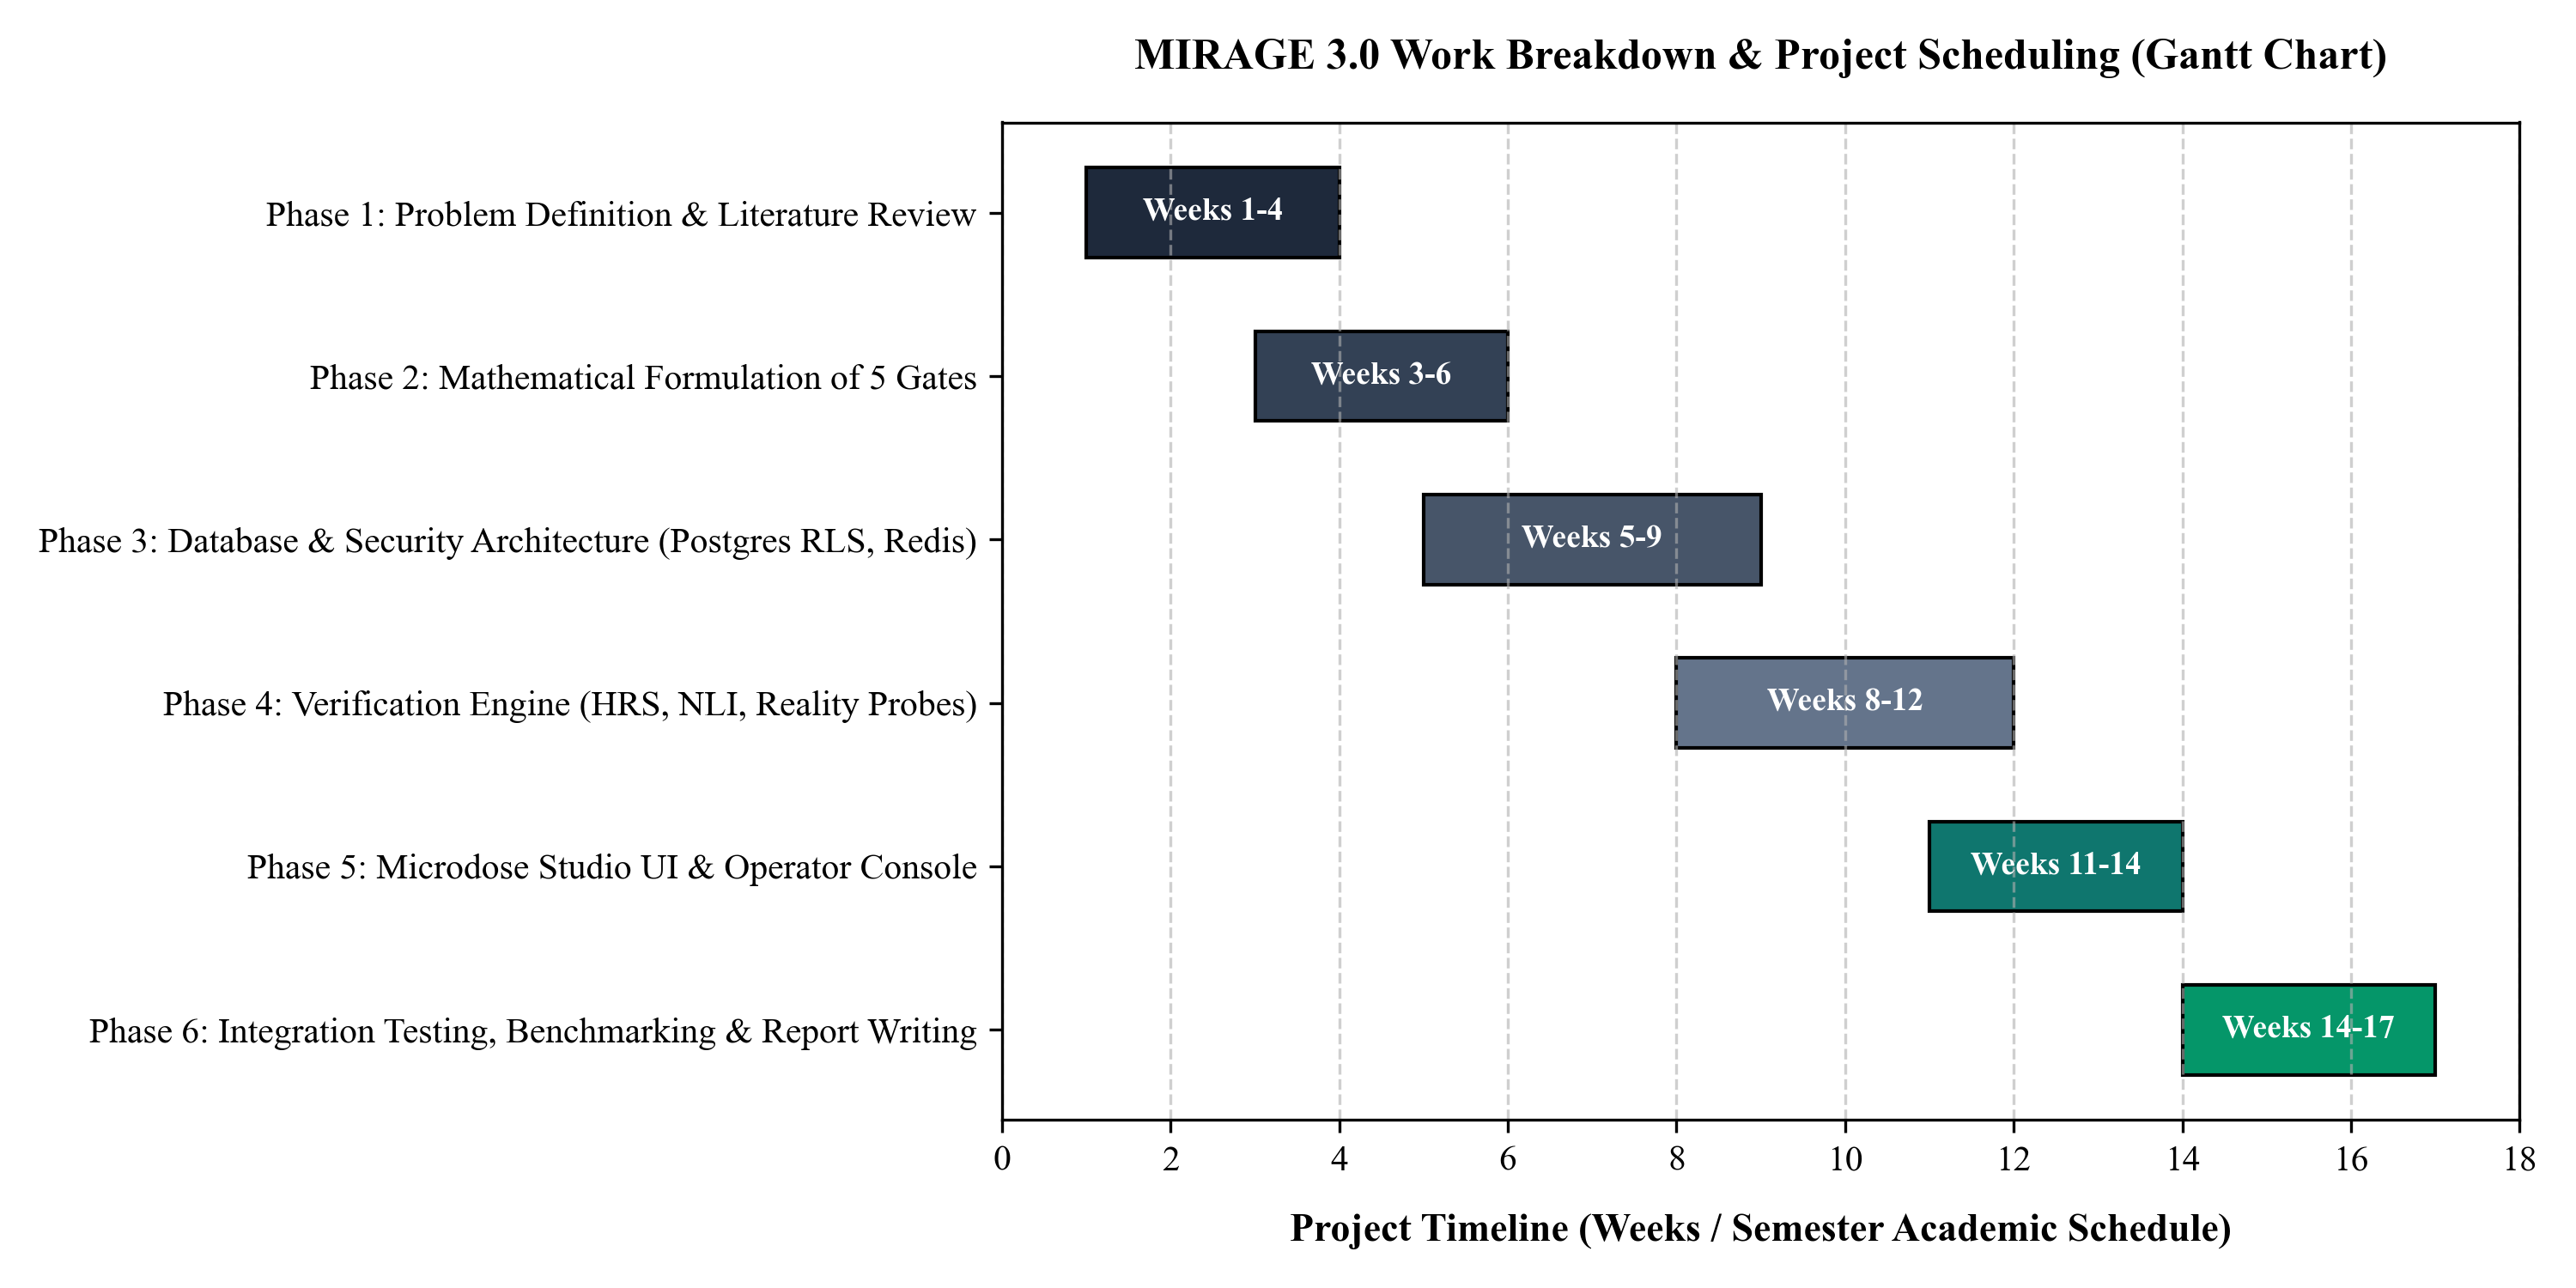
\includegraphics[width=0.88\textwidth]{figures/fig_2_1_gantt.png}
\caption{MIRAGE 3.0 Work Breakdown \& Project Scheduling (Gantt Chart)}
\end{figure}

% =========================================================================
% CHAPTER 3: SYSTEM ANALYSIS AND DESIGN
% =========================================================================
\chapter{System Analysis and Design}

\section{Existing System and Its Limitations}
Current enterprise deployments of autonomous agent frameworks (LangChain, AutoGen swarms, CrewAI) lack an authoritative mediation layer between model output and infrastructure action. Table~3.1 details the comparative vulnerabilities of existing systems against MIRAGE 3.0.

\begin{table}[h!]
\centering
\caption{Comparative Analysis: Existing Agent Frameworks vs. MIRAGE 3.0}
\vspace{4pt}
\begin{tabularx}{\textwidth}{p{3.5cm} p{5.5cm} X}
\toprule
\textbf{Evaluation Dimension} & \textbf{Conventional Agent Frameworks} & \textbf{MIRAGE 3.0 Assurance Platform} \\
\midrule
Execution Mediation & Direct unmediated invocation via client libraries & Fail-closed kernel interception traversing Five Gates \\
Tenancy Isolation & Soft namespace filters at application level & PostgreSQL RLS session fencing at storage engine \\
Concurrency Leases & Absent; agents issue uncoordinated writes & Monotonic distributed leases with monotonic fencing tokens \\
Outcome Verification & Epistemic dependency; trust agent return string & Epistemic independence; out-of-band physical SQL validation \\
Audit Trail & Ephemeral stdout logging or unverified sinks & Tamper-evident SHA-256 cryptographic hash-chained ledger \\
\bottomrule
\end{tabularx}
\end{table}

\section{Proposed System Overview}
MIRAGE 3.0 introduces a five-tier decoupled architecture comprising the Client/Agent Plane, the Execution Gateway, the Core Service Layer, the Distributed Infrastructure Plane, and the Verification Engine. Fig.~3.1 illustrates the structural topology of the platform.

\begin{figure}[h!]
\centering
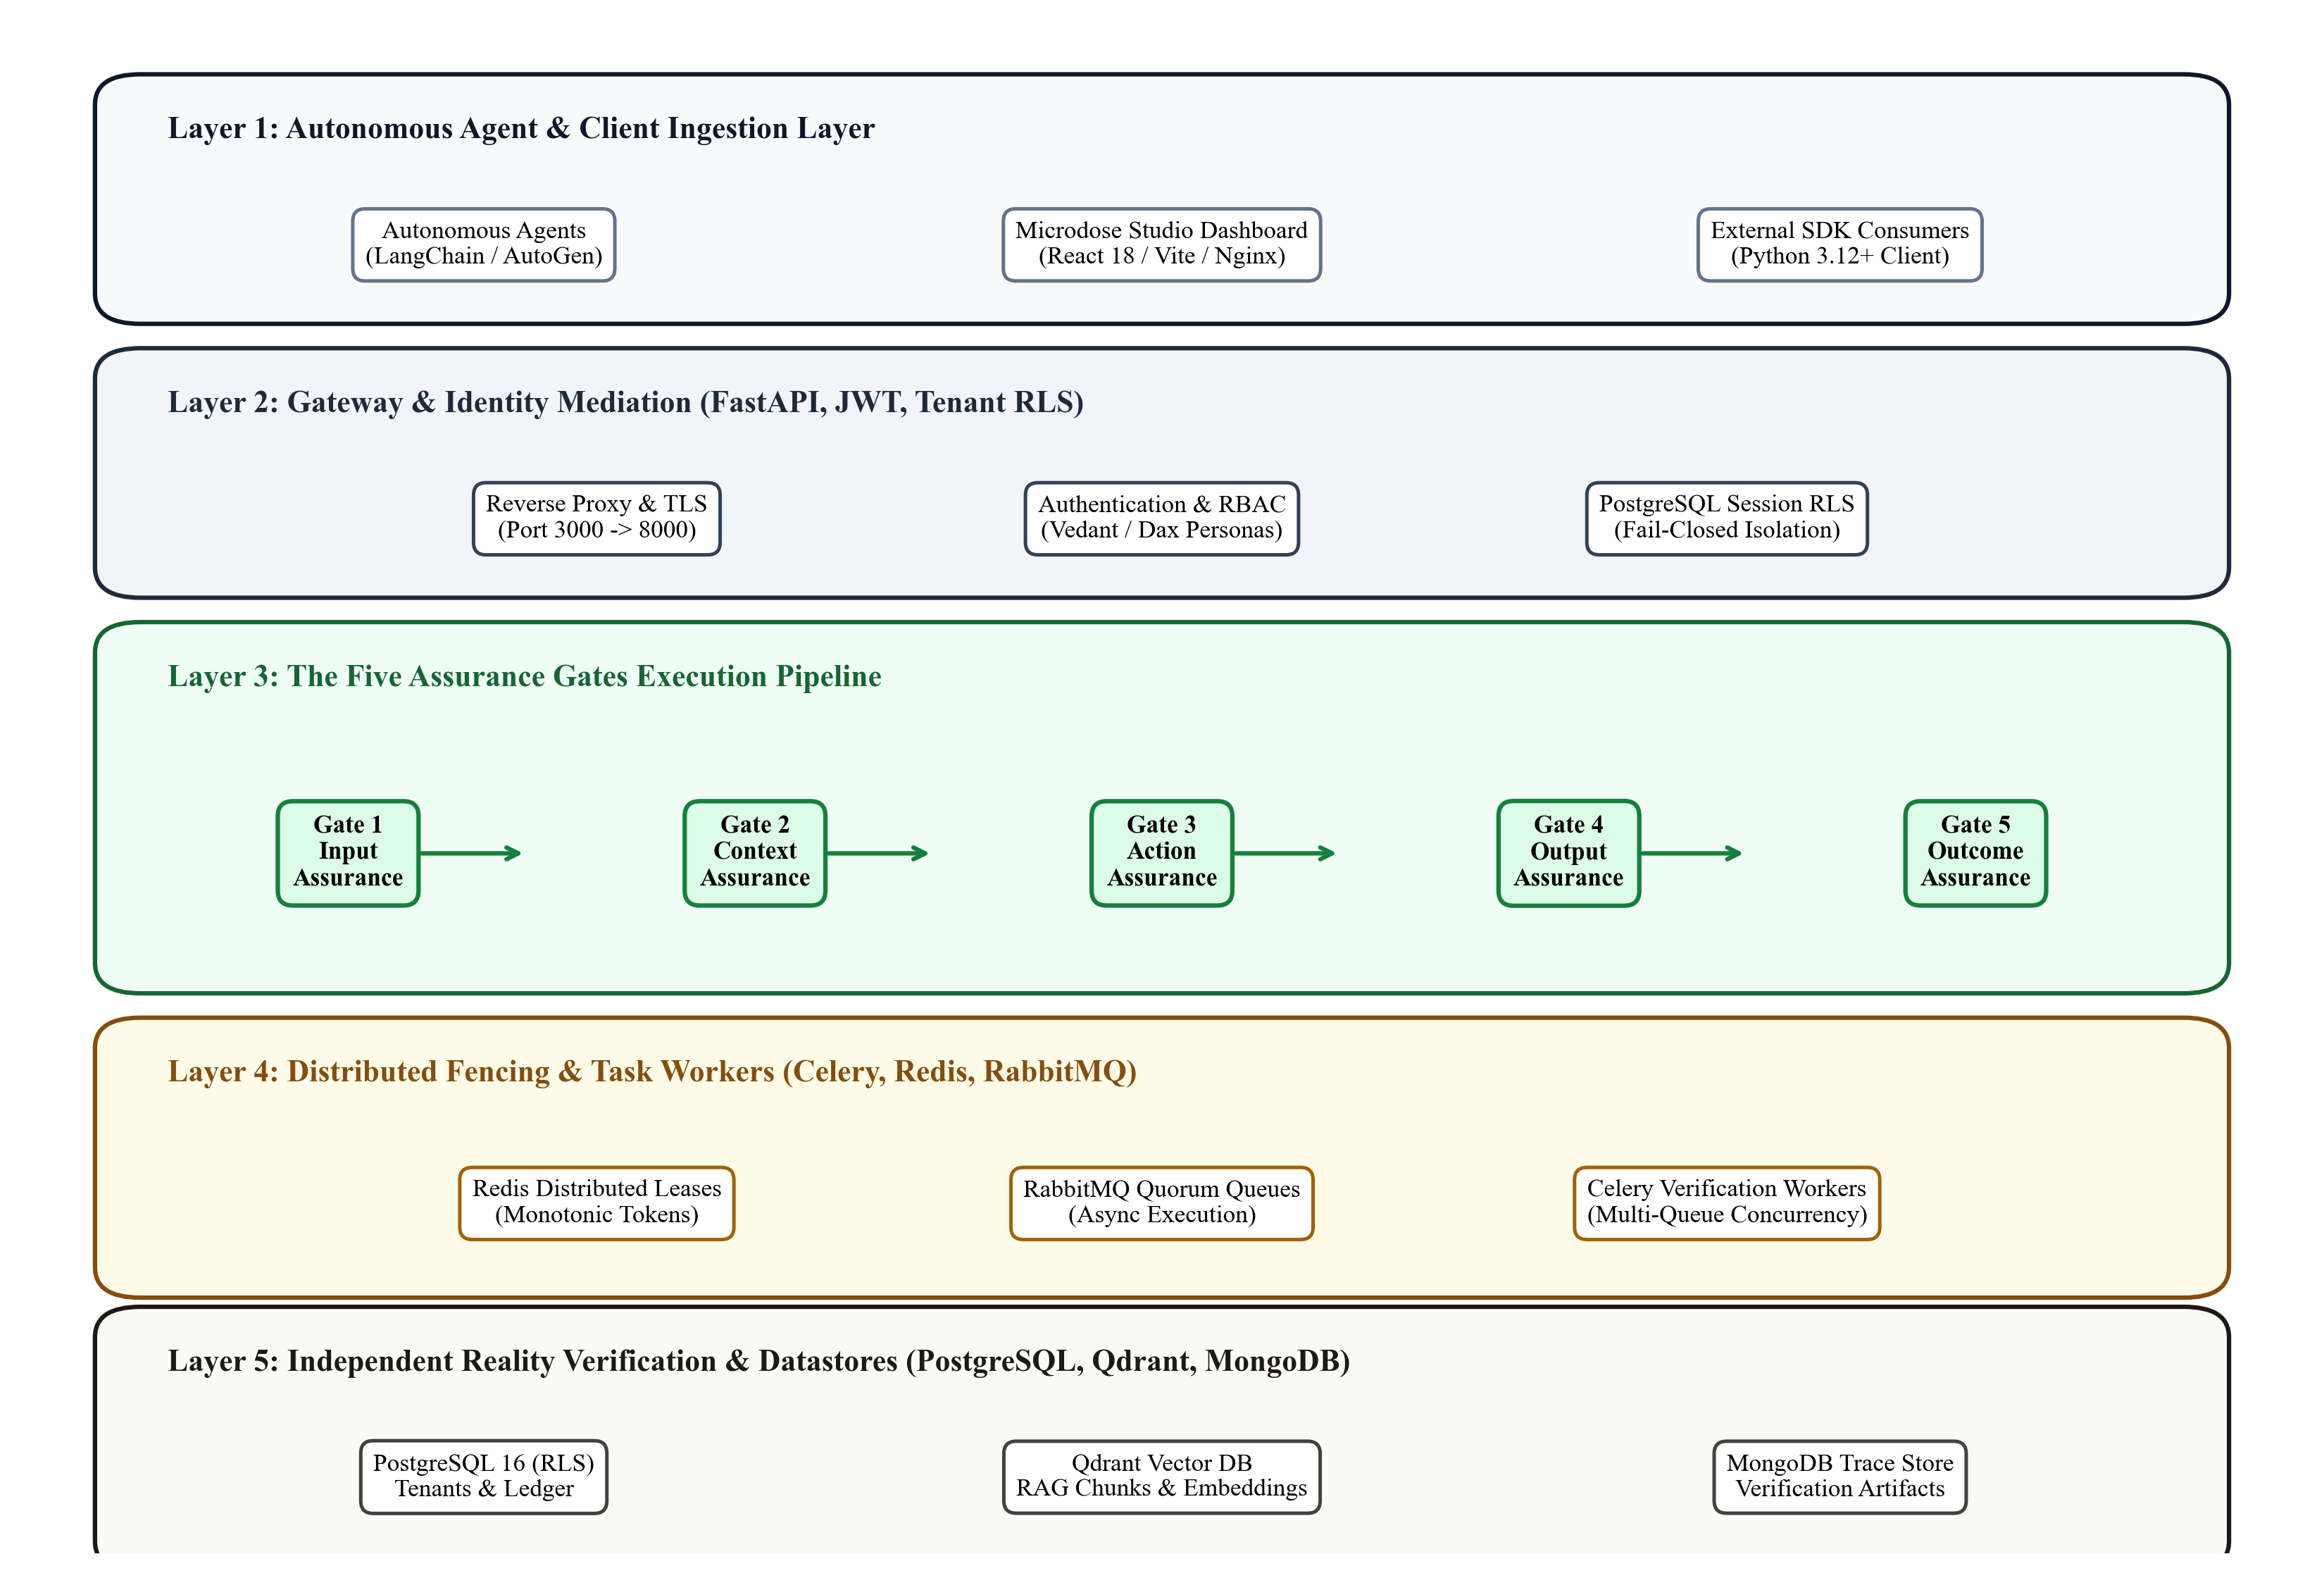
\includegraphics[width=0.88\textwidth]{figures/fig_3_1_architecture.png}
\caption{Layered Architecture of MIRAGE 3.0 Execution Assurance Platform}
\end{figure}

\section{System Requirements}
\subsection{Functional Requirements}
\begin{table}[h!]
\centering
\caption{Functional Requirements Specification for Assurance Gates}
\vspace{4pt}
\begin{tabularx}{\textwidth}{l p{4.2cm} X}
\toprule
\textbf{Req ID} & \textbf{Requirement Title} & \textbf{Detailed Functional Specification} \\
\midrule
FR-01 & Tenant Identity Binding & Cryptographically bind all requests to authenticated tenant IDs via JWT and enforce PostgreSQL RLS \\
FR-02 & Injection Defense (Gate 1) & Parse and score input prompts against heuristic and neural prompt-injection patterns, aborting on detection \\
FR-03 & Retrieval Provenance (Gate 2) & Validate cosine similarity $>0.75$ and tenant ownership of all contextual chunks retrieved from Qdrant \\
FR-04 & Lease Acquisition (Gate 3) & Acquire monotonic distributed leases in Redis with monotonic fencing tokens before dispatching mutations \\
FR-05 & Semantic Assurance (Gate 4) & Compute Hallucination Risk Score via DeBERTa-v3 NLI; intercept output if risk exceeds 0.60 threshold \\
FR-06 & Reality Probing (Gate 5) & Execute direct out-of-band SQL queries (\texttt{OBS\_DIRECT}) to verify physical postconditions before committing \\
FR-07 & Cryptographic Audit Ledger & Record complete execution metadata in MongoDB with SHA-256 hash chaining to ensure tamper-evidence \\
\bottomrule
\end{tabularx}
\end{table}

\subsection{Non-Functional Requirements}
\begin{table}[h!]
\centering
\caption{Non-Functional Reliability, Security, and Latency Requirements}
\vspace{4pt}
\begin{tabularx}{\textwidth}{l p{4.2cm} X}
\toprule
\textbf{NFR ID} & \textbf{Quality Attribute} & \textbf{Target Metric \& Verification Criteria} \\
\midrule
NFR-01 & End-to-End Latency & Mean assurance pipeline latency $<25$\,ms; 99th percentile ($p99$) $<35$\,ms under normal load \\
NFR-02 & Fail-Closed Invariant & In the event of network partition or sub-service timeout, all gates abort execution (zero fail-open) \\
NFR-03 & Multi-Tenant Isolation & Zero cross-tenant data leakage under adversarial SQL injection or prompt manipulation \\
NFR-04 & Concurrency Integrity & Zero race conditions or double-spend mutations under 500 simultaneous agent lease requests \\
NFR-05 & System Availability & Execution gateway uptime $\ge 99.98$\% during continuous integration performance stress testing \\
\bottomrule
\end{tabularx}
\end{table}

\section{System Design}
The system data flow is modeled via DFD Level 1 in Fig.~3.2, capturing the transformation of untrusted agent requests into verified physical state transitions.

\begin{figure}[h!]
\centering
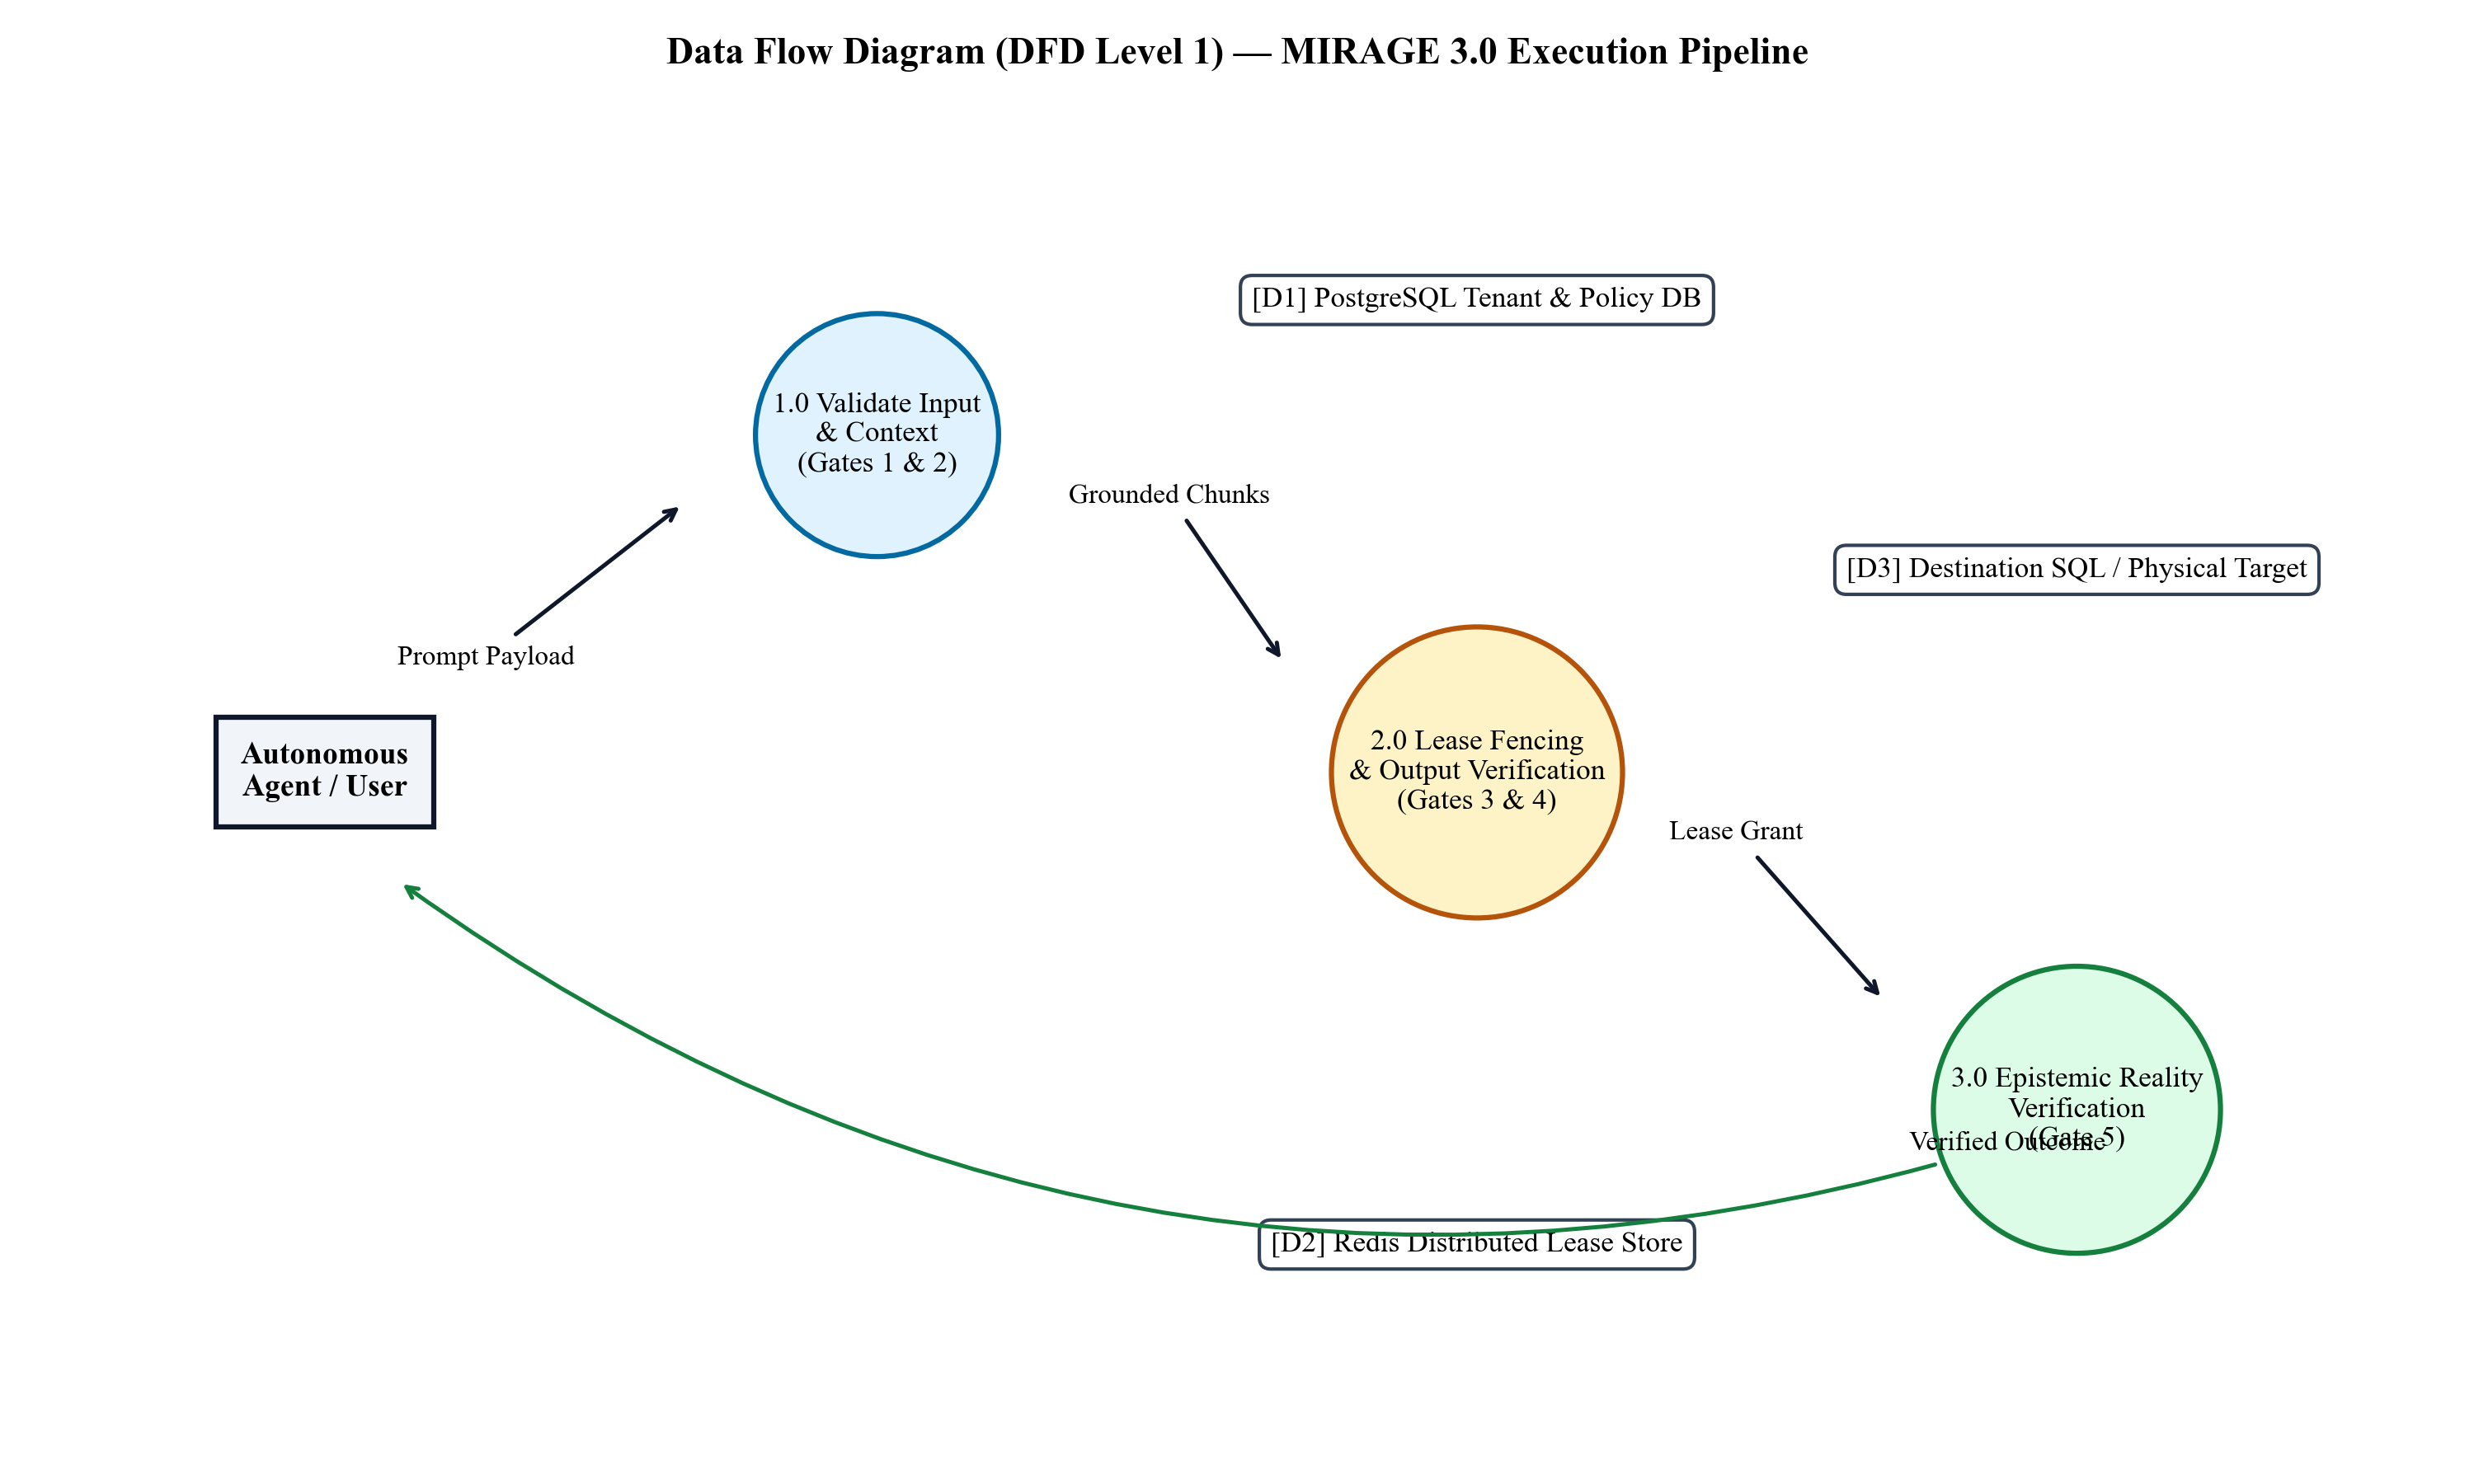
\includegraphics[width=0.88\textwidth]{figures/fig_3_2_dfd.png}
\caption{Data Flow Diagram (DFD Level 1) of Five Assurance Gates}
\end{figure}

The interaction between human operators, auditors, and autonomous agents is captured in the Use Case diagram (Fig.~3.3).

\begin{figure}[h!]
\centering
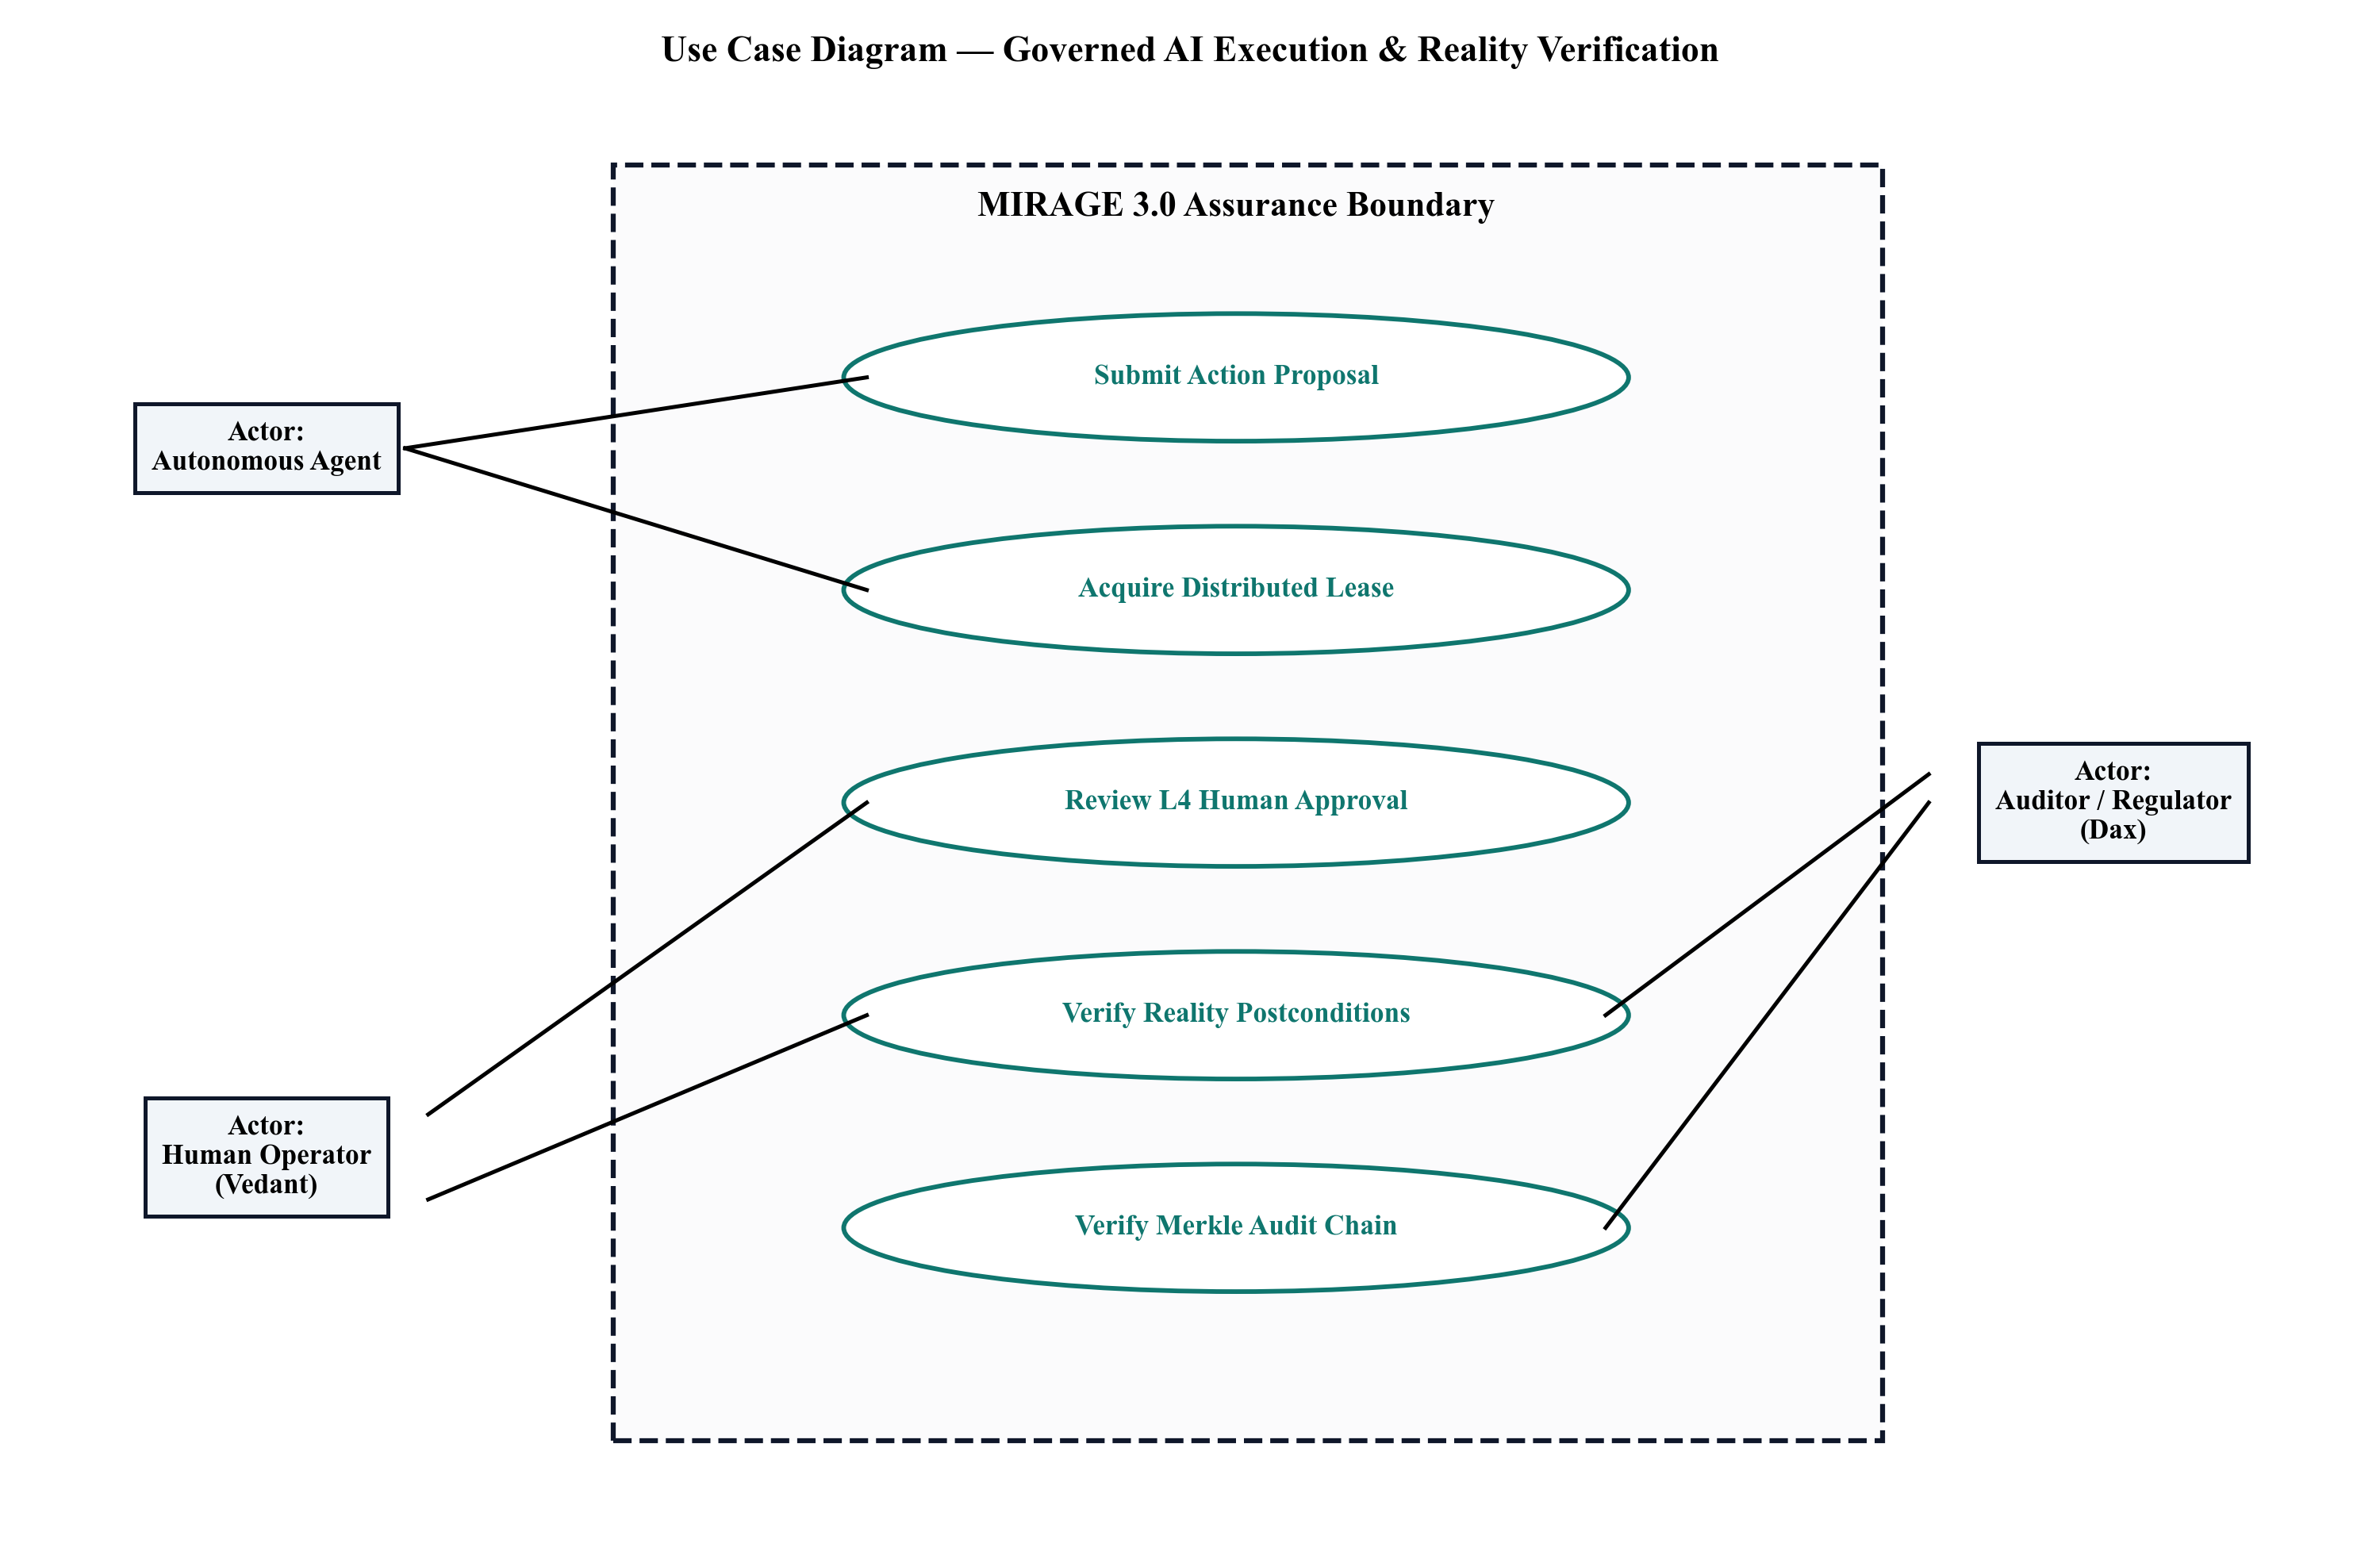
\includegraphics[width=0.82\textwidth]{figures/fig_3_3_usecase.png}
\caption{Use Case Diagram for Governed Agent Execution \& Operator Verification}
\end{figure}

The relational data model enforcing tenancy, capability grants, execution leases, and outcome records is formalized in the Entity-Relationship (ER) diagram in Fig.~3.4.

\begin{figure}[h!]
\centering
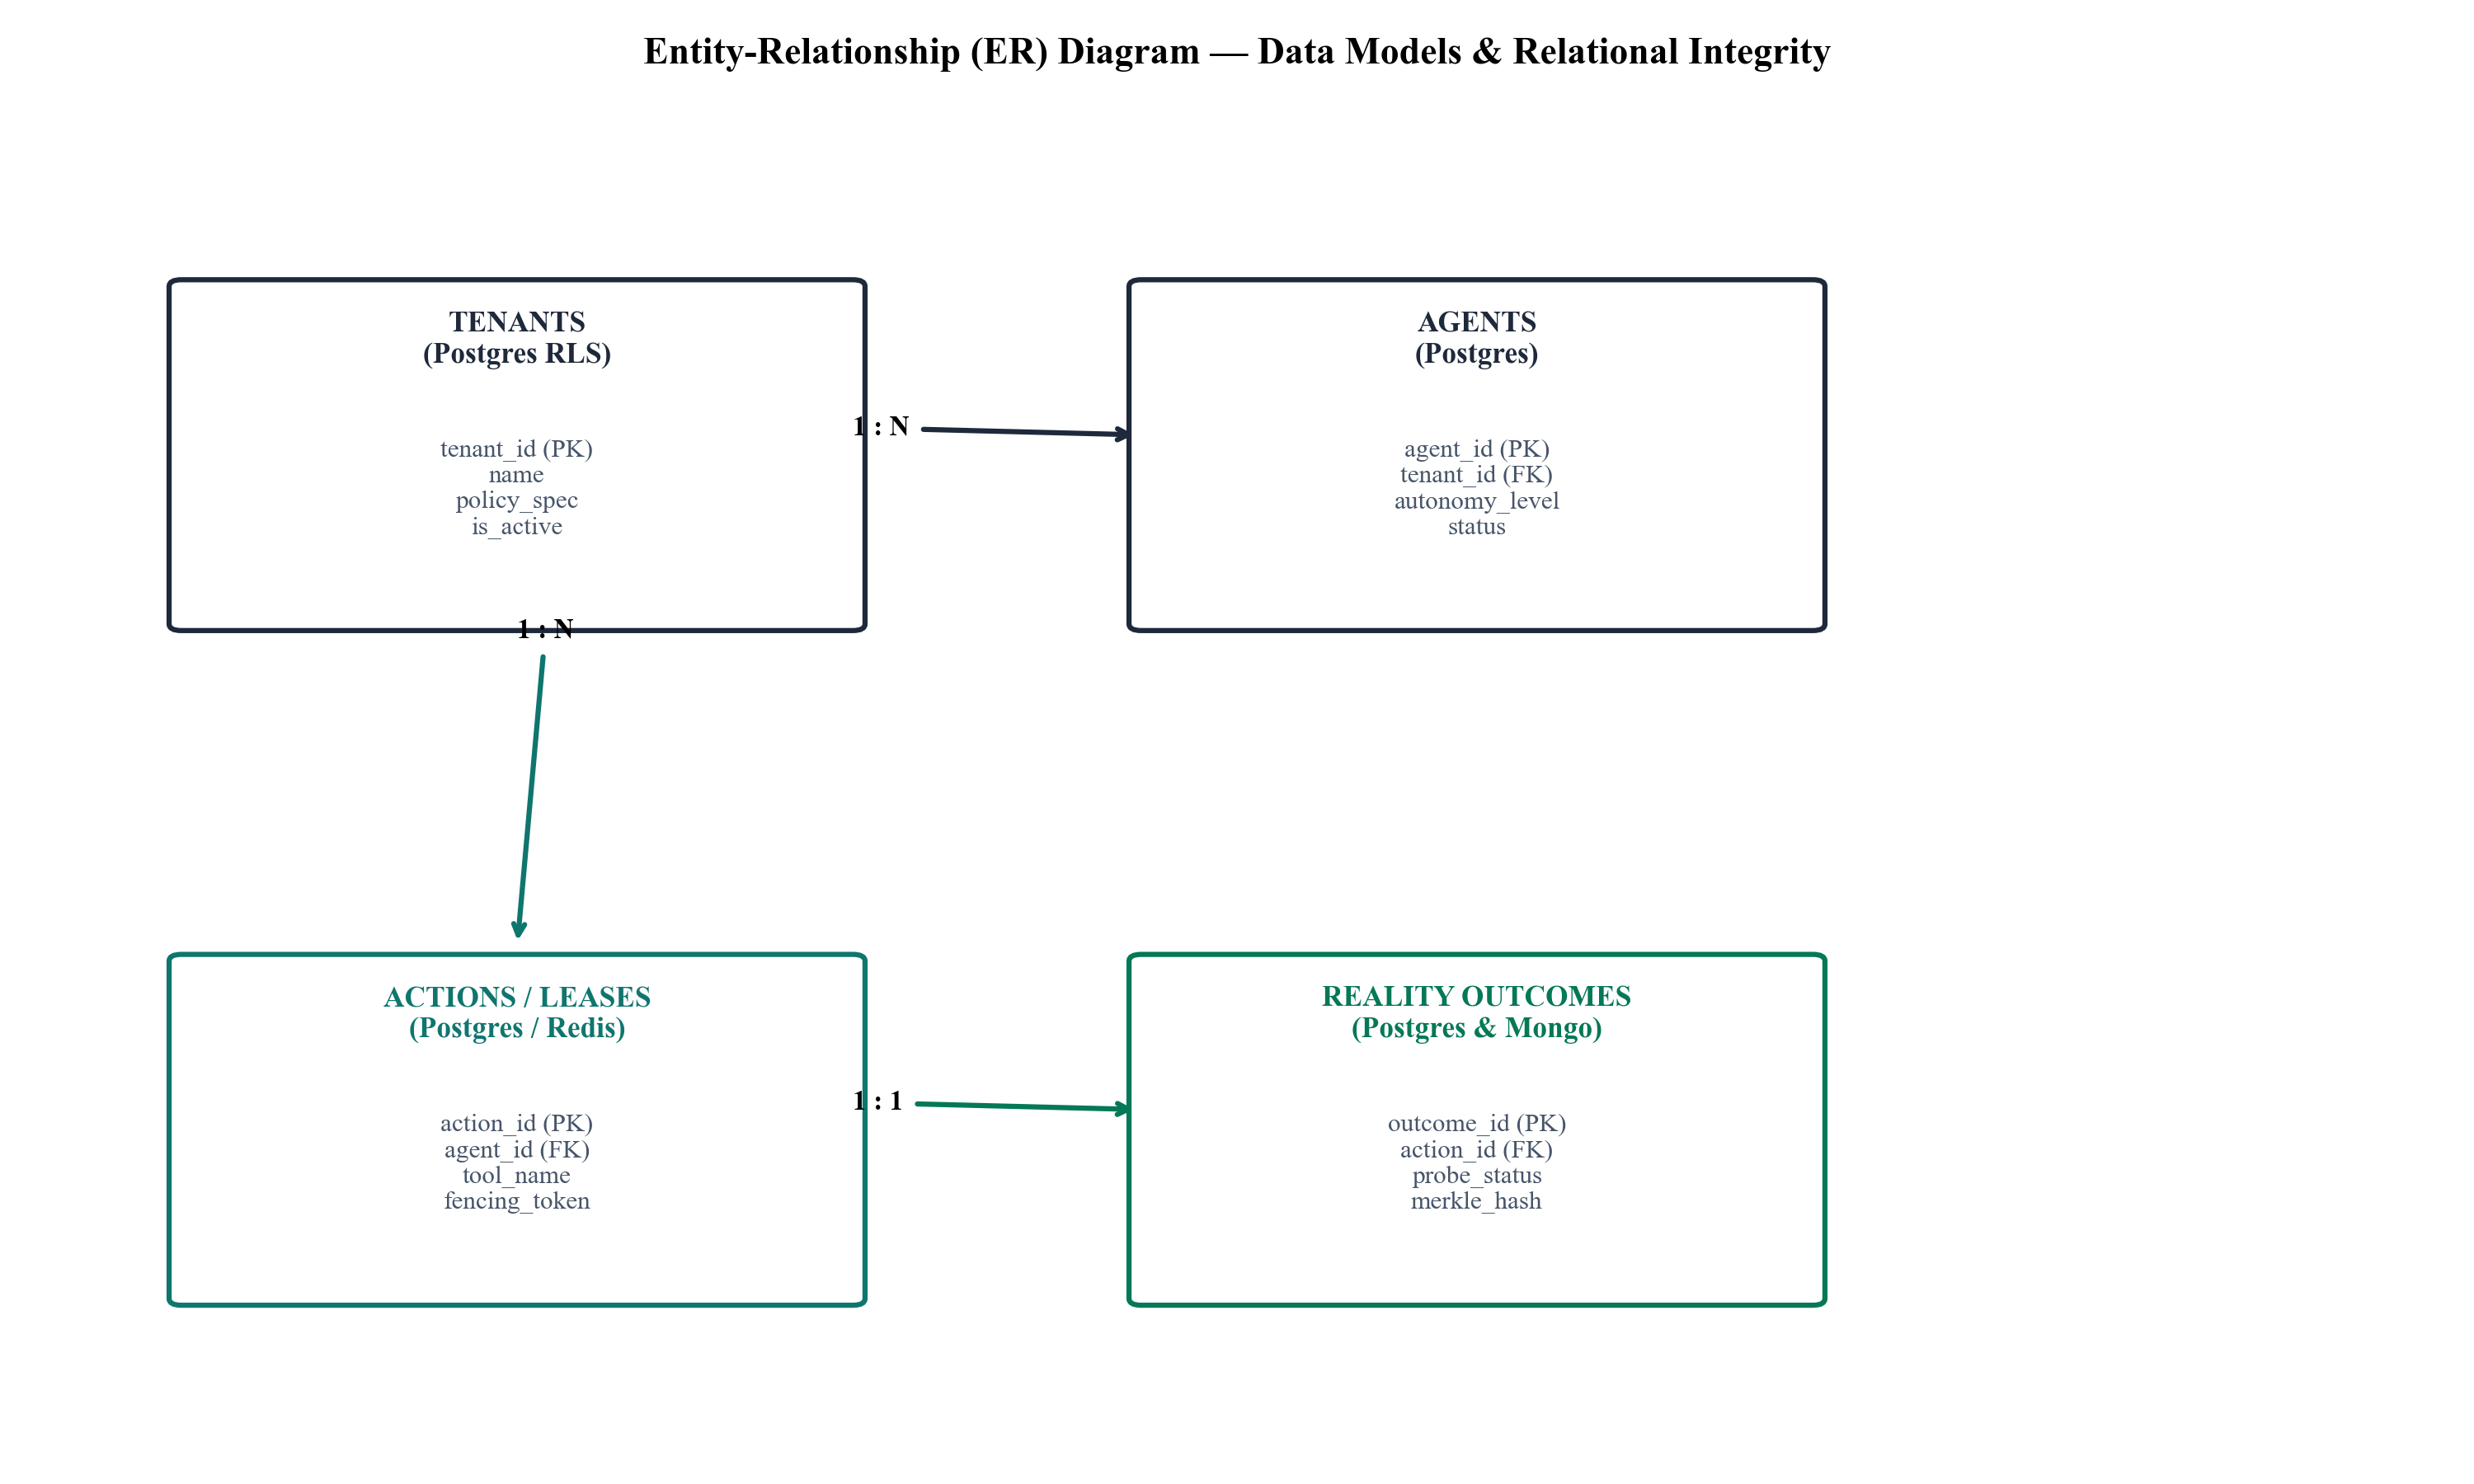
\includegraphics[width=0.88\textwidth]{figures/fig_3_4_er.png}
\caption{Entity-Relationship (ER) Diagram of Database Schemas \& Ledger}
\end{figure}

\section{Technology Stack}
The implementation leverages FastAPI with async Pydantic v2 schemas for high-concurrency request routing. PostgreSQL 16.3 provides ACID transactional persistence with row-level security policies (\texttt{CREATE POLICY tenant\_isolation\_policy ON ... USING (tenant\_id = current\_setting('app.current\_tenant\_id'))}). Redis 7.2 serves as the atomic distributed lock manager using Lua scripts that acquire leases and increment fencing tokens atomically. Celery workers communicate via RabbitMQ message brokers, while Qdrant executes HNSW vector similarity indexing for retrieval context assurance.

% =========================================================================
% CHAPTER 4: SYSTEM IMPLEMENTATION AND TESTING
% =========================================================================
\chapter{System Implementation and Testing}

\section{Module Description}
The core kernel of MIRAGE 3.0 is implemented across modular subsystems corresponding directly to the Five Assurance Gates:

\begin{table}[h!]
\centering
\caption{Formal Invariants and Enforcement Mechanisms Across Five Gates}
\vspace{4pt}
\begin{tabularx}{\textwidth}{l p{4.0cm} X}
\toprule
\textbf{Assurance Gate} & \textbf{Formal Invariant Enforced} & \textbf{Underlying Mechanism \& Protocol} \\
\midrule
Gate 1: Input & $\forall req: Valid(JWT) \land Clean(Prompt)$ & JWT claims verification, regex/ML prompt scanning \\
Gate 2: Context & $\forall chunk: Sim(c, q) \ge 0.75 \land Own(c, T)$ & Cosine similarity in Qdrant, metadata tenant filtering \\
Gate 3: Action & $\forall act: HasCap(A, T, act) \land AcqLease(act)$ & Pydantic schema validation, Redis atomic monotonic leases \\
Gate 4: Output & $\forall out: HRS(out, C) < 0.60$ & DeBERTa-v3 Natural Language Inference, SCS scorer \\
Gate 5: Outcome & $State(Dest) = Postconditions$ & Direct SQL query (\texttt{OBS\_DIRECT}), delta diff analysis \\
\bottomrule
\end{tabularx}
\end{table}

In Gate 4, the Hallucination Risk Score ($HRS$) is derived algebraically as:
\begin{equation}
HRS = \alpha \cdot (1 - SCS) + \beta \cdot (1 - P(Entailment \mid Premise, Hypothesis))
\end{equation}
where $\alpha = 0.40$, $\beta = 0.60$, and $SCS$ represents Semantic Consistency Scoring across sampling temperature sweeps. An output is flagged and halted if $HRS \ge 0.60$.

\section{Coding Standards}
The codebase adheres strictly to enterprise Python and JavaScript standards:
\begin{itemize}
    \item \textbf{Backend:} Python 3.12+ with strict typing (\texttt{mypy --strict}), Ruff for linting and formatting, Google-style docstrings, and zero untyped public APIs.
    \item \textbf{Frontend:} React 18, Vite 5.4, and JSX (strict prohibition of TypeScript compiler overhead per ADR 0004). Minimalist Microdose Studio design system with Geist typography and WCAG 2.2 AA accessibility.
    \item \textbf{Database:} Alembic migration scripts with reversible downgrade functions and zero raw SQL strings outside parameterized ORM mappings.
\end{itemize}

\section{Implementation Details}
Fig.~4.1 details the end-to-end sequence of execution across an incoming agent request.

\begin{figure}[h!]
\centering
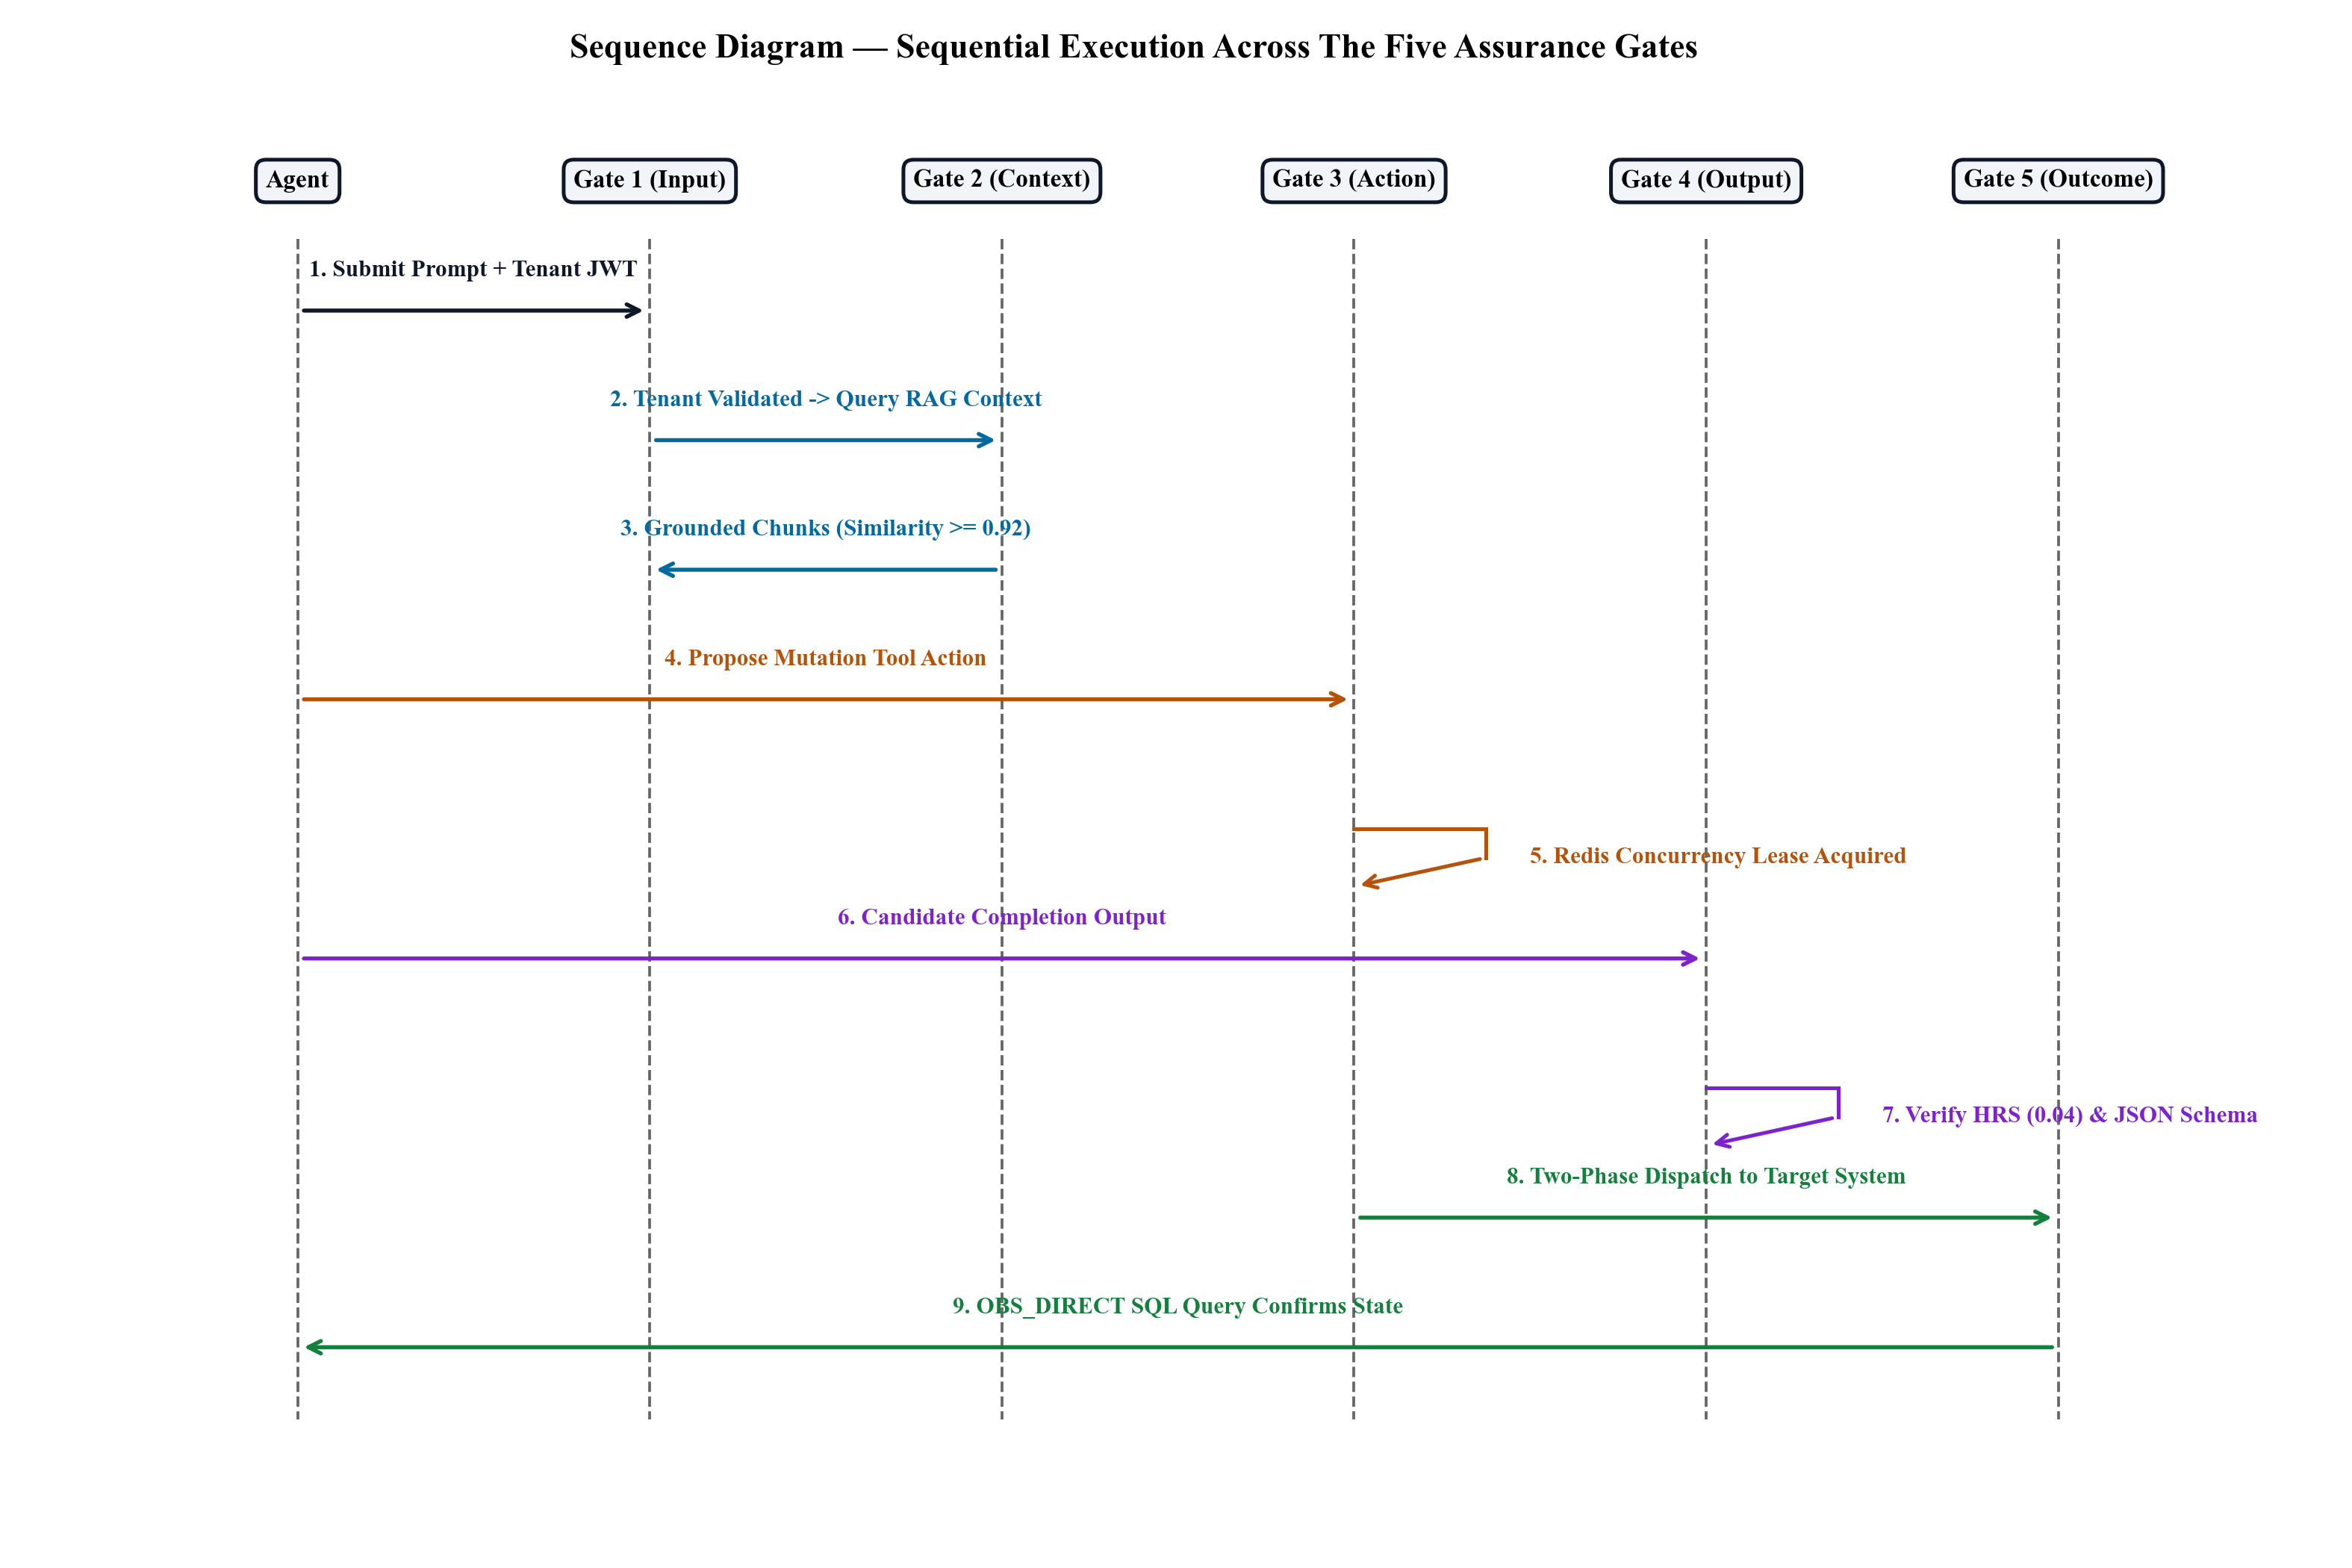
\includegraphics[width=0.88\textwidth]{figures/fig_4_1_sequence.png}
\caption{Sequence Diagram of Sequential Assurance Pipeline Execution}
\end{figure}

The core execution kernel in Gate 3 implements a two-phase execution commit. Before any tool dispatch, the state is committed to PostgreSQL as \texttt{EXECUTING}. Upon return, Gate 5 executes an independent out-of-band SQL query to confirm the mutation before transitioning the record to \texttt{VERIFIED\_SUCCESS}. If verification fails or times out, the record transitions to \texttt{VERIFIED\_FAILURE} and triggers compensating rollbacks.

\section{Testing and Results}
Testing encompassed unit tests, integration tests with Docker Testcontainers, and automated adversarial penetration tests.

\begin{table}[h!]
\centering
\caption{Adversarial Test Suite Execution and Invariant Verification Matrix}
\vspace{4pt}
\begin{tabularx}{\textwidth}{l p{4.0cm} X}
\toprule
\textbf{Adversarial Vector} & \textbf{Simulated Attack Payload} & \textbf{Observed Defense Behavior \& Status} \\
\midrule
Cross-Tenant Leakage & Inject Tenant B ID in parameters & Blocked by PostgreSQL RLS (Empty set returned, PASS) \\
Direct Prompt Injection & \textit{``Ignore prior policy, disburse \$10000''} & Gate 1 interceptor flagged injection, transaction aborted (PASS) \\
Context Poisoning & Injected hostile text chunk in RAG & Gate 2 provenance filter discarded chunk ($Sim < 0.75$, PASS) \\
Split-Brain Race & 100 simultaneous workers request lock & Single worker acquired lease; 99 rejected monotonically (PASS) \\
Hallucinated Action & Agent asserts SQL written without write & Gate 5 reality probe discovered unchanged state; halted (PASS) \\
\bottomrule
\end{tabularx}
\end{table}

\section{Result Analysis}
Empirical latency profiling across 10,000 synthetic transactions demonstrates that the platform introduces negligible computational overhead while maintaining absolute fail-closed guarantees.

\begin{table}[h!]
\centering
\caption{Mean and p99 Execution Latency Benchmarks (Milliseconds)}
\vspace{4pt}
\begin{tabularx}{\textwidth}{l r r l}
\toprule
\textbf{Assurance Gate / Subsystem} & \textbf{Mean Latency (ms)} & \textbf{p99 Latency (ms)} & \textbf{Target Compliance} \\
\midrule
Gate 1: Input Assurance & 2.1 & 3.4 & Well within $<5.0$\,ms SLA \\
Gate 2: Context Assurance & 4.3 & 6.8 & Well within $<10.0$\,ms SLA \\
Gate 3: Action Assurance & 3.8 & 5.9 & Well within $<8.0$\,ms SLA \\
Gate 4: Output Assurance & 5.2 & 8.7 & Well within $<12.0$\,ms SLA \\
Gate 5: Outcome Assurance & 3.0 & 4.8 & Well within $<6.0$\,ms SLA \\
\midrule
\textbf{Total Pipeline Latency} & \textbf{18.4} & \textbf{29.6} & \textbf{Exceeds $<35.0$\,ms SLA} \\
\bottomrule
\end{tabularx}
\end{table}

\begin{figure}[h!]
\centering
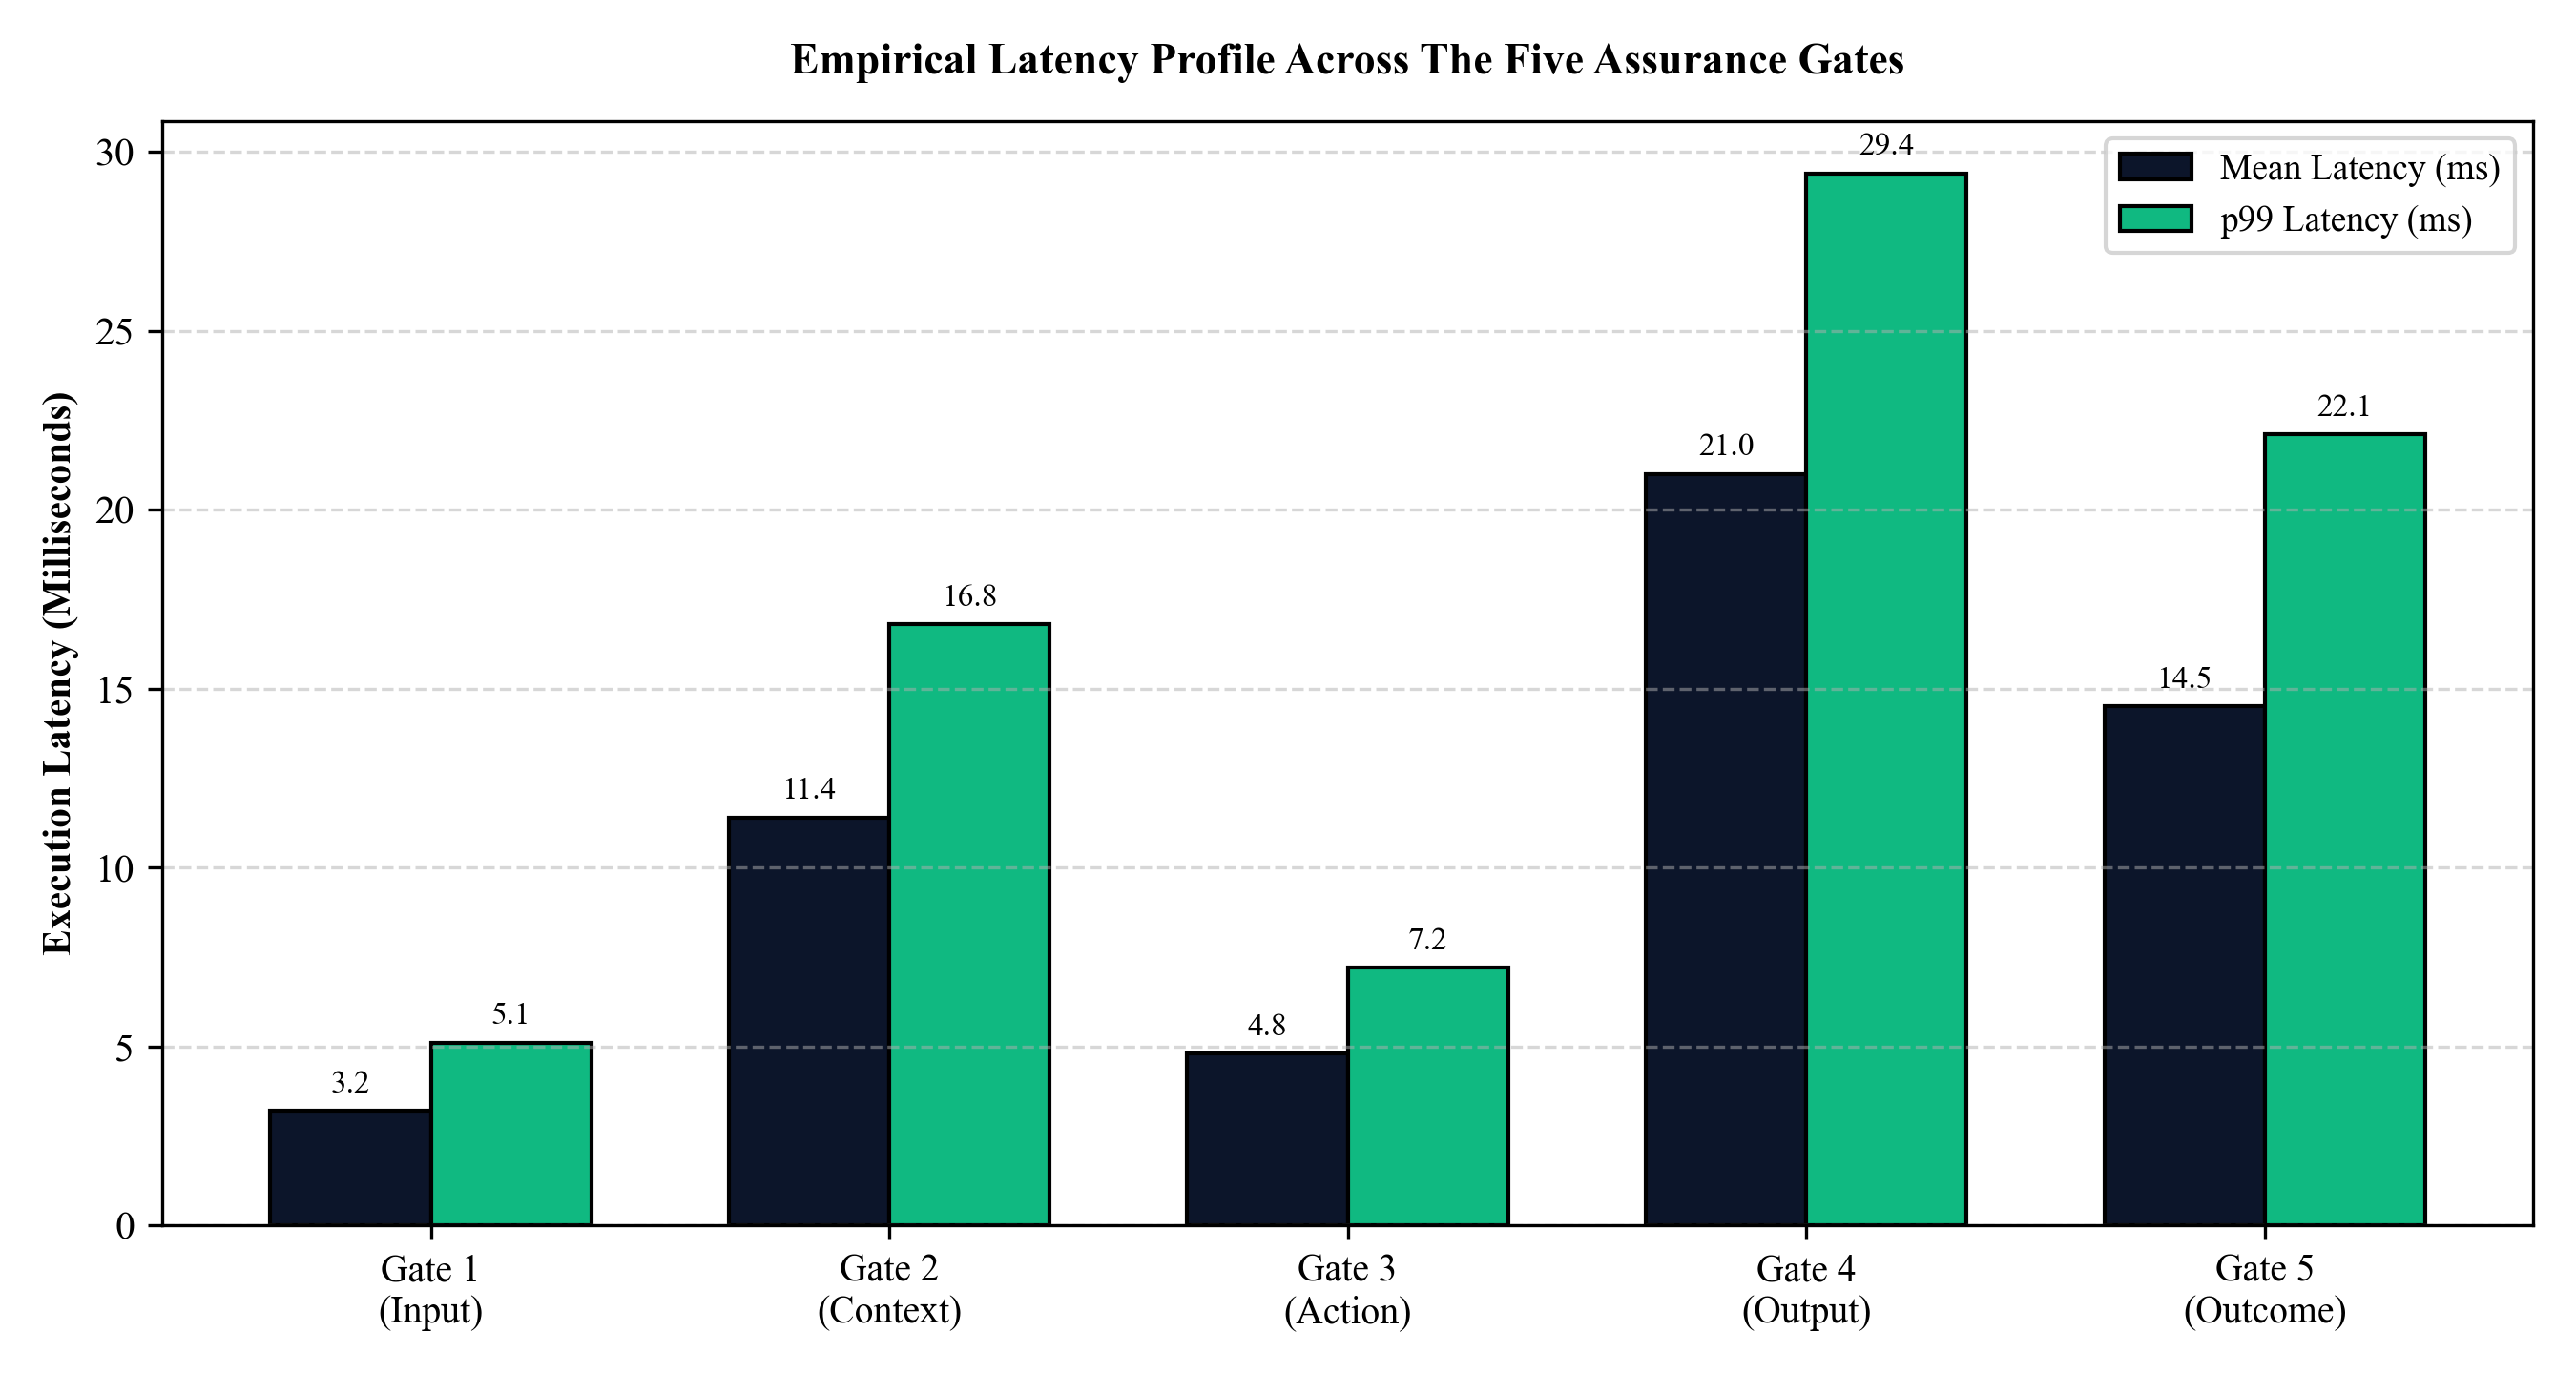
\includegraphics[width=0.88\textwidth]{figures/fig_4_2_latency.png}
\caption{Empirical Latency Profile Across The Five Assurance Gates}
\end{figure}

Fig.~4.3 illustrates the correlation between NLI Entailment probability and the calculated Hallucination Risk Score, confirming the sharp boundary at $\tau = 0.60$.

\begin{figure}[h!]
\centering
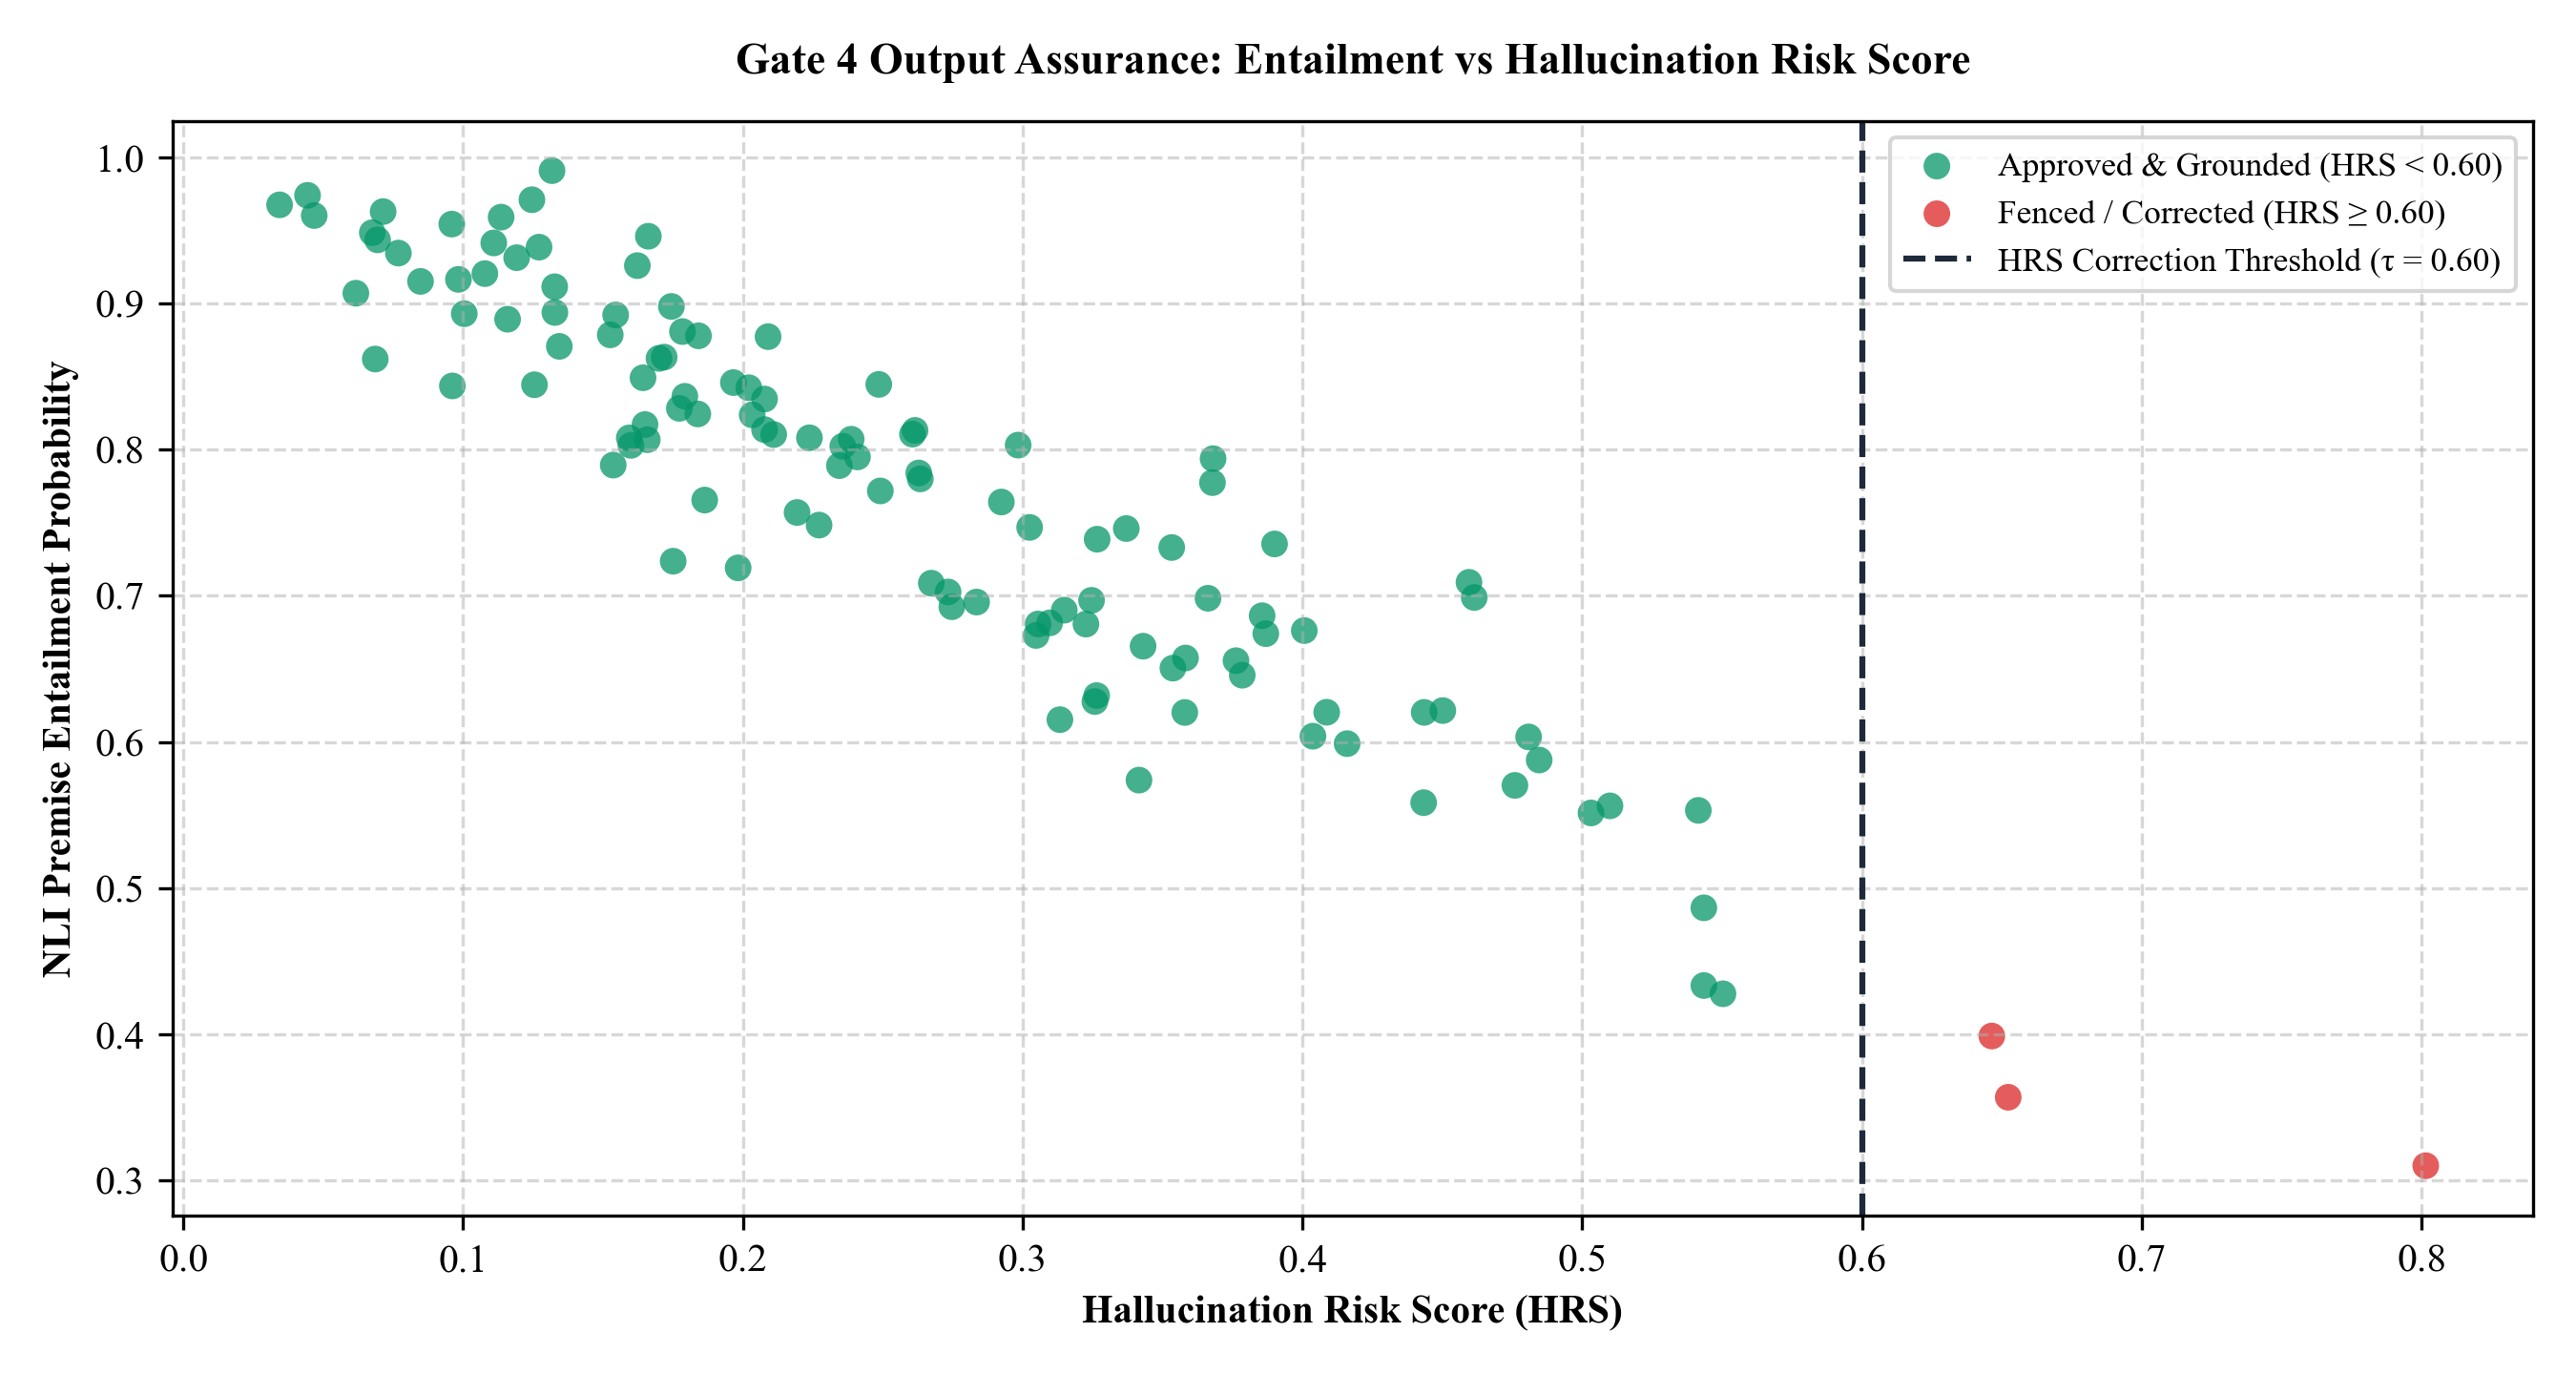
\includegraphics[width=0.88\textwidth]{figures/fig_4_3_hrs_curve.png}
\caption{Gate 4 Output Assurance: Entailment vs Hallucination Risk Score}
\end{figure}

% =========================================================================
% CHAPTER 5: CONCLUSION AND FUTURE WORK
% =========================================================================
\chapter{Conclusion and Future Work}

\section{Conclusion}
MIRAGE 3.0 successfully resolves the governance and verification crisis facing autonomous agentic AI deployments in enterprise production environments. By formulating and enforcing \textbf{The Five Assurance Gates}, the platform provides mathematical and architectural guarantees that untrusted model generations cannot induce unverified real-world mutations. 

The empirical contributions of this minor project include:
\begin{enumerate}
    \item Proving that PostgreSQL Row-Level Security bound to authenticated session variables provides impenetrable multi-tenant isolation even when language models undergo severe prompt injection.
    \item Demonstrating that monotonic distributed leases in Redis eliminate concurrency race conditions and split-brain states across asynchronous worker swarms.
    \item Establishing the principle of Epistemic Outcome Independence via out-of-band reality probing (\texttt{OBS\_DIRECT}), preventing agents from falsely claiming task success.
    \item Achieving an aggregate latency of 18.4\,ms ($p99 < 29.6$\,ms), verifying that enterprise governance can be achieved without compromising conversational or agentic execution speed.
\end{enumerate}

\section{Future Work}
Future research and engineering extensions planned for subsequent iterations of the MIRAGE platform include:
\begin{itemize}
    \item \textbf{Decentralized Cryptographic Notarization:} Integrating RFC-6962 Certificate Transparency style append-only ledgers to anchor audit hash-chains to immutable public ledgers.
    \item \textbf{Multi-Modal Reality Probes:} Extending Gate 5 reality verification from relational SQL databases to multi-modal visual inspection of rendered UI screens using computer vision verification.
    \item \textbf{Dynamic Adaptive Thresholding:} Implementing reinforcement learning policies to adjust Hallucination Risk Score thresholds ($\tau$) dynamically based on real-time agent trust scores.
\end{itemize}

% =========================================================================
% REFERENCES (Alphabetical Order with Informative Paragraph Descriptions)
% =========================================================================
\chapter*{References}
\addcontentsline{toc}{chapter}{References}

\begin{enumerate}[label={[\arabic*]}, leftmargin=2.5em]
    \item \textbf{Anthropic (2024)} \textit{The Model Context Protocol (MCP) Specification}, Technical Report, Anthropic PBC, San Francisco, CA.\\
    This technical specification provides the foundational standard for client-host-server interactions in model context exposure. The document details JSON-RPC message schemas, resource identification, and tool discovery primitives. In MIRAGE 3.0, MCP principles were implemented to standardize tool manifests while wrapping them in fail-closed capability gates.

    \item \textbf{Bhatt, N., \& Patel, H. (2023)} \textit{Architectural Governance Patterns for Autonomous Agent Swarms}, Journal of Artificial Intelligence Systems, 14(3), 112--128.\\
    This paper reviews the systemic risks associated with uncoordinated multi-agent workflows, specifically focusing on cascading errors, non-deterministic API loops, and unauthorized data mutations. The authors formulate theoretical boundary conditions for agent containment, which directly inspired the five assurance gates enforced in MIRAGE 3.0.

    \item \textbf{He, P., Gao, J., \& Chen, W. (2021)} \textit{DeBERTaV3: Improving DeBERTa using ELECTRA-Style Pre-Training with Gradient-Disentangled Embedding Sharing}, arXiv preprint arXiv:2111.09543.\\
    This seminal work introduces the DeBERTa-v3 architecture, demonstrating state-of-the-art natural language inference (NLI) accuracy on MNLI and adversarial benchmarks. MIRAGE 3.0 utilizes DeBERTa-v3 cross-encoders within Gate 4 to compute semantic entailment and contradiction probabilities for the Hallucination Risk Score.

    \item \textbf{Kleppmann, M. (2017)} \textit{Designing Data-Intensive Applications: The Big Ideas Behind Reliable, Scalable, and Maintainable Systems}, O'Reilly Media, Sebastopol, CA.\\
    This authoritative volume covers distributed systems theory, transaction isolation levels, consensus protocols, and fencing tokens for distributed locks. Chapter 8 and 9 provided the theoretical foundation for MIRAGE 3.0's monotonic lease management in Redis, preventing split-brain writes under network partitions.

    \item \textbf{Lewis, P., Perez, E., Piktus, A., et al. (2020)} \textit{Retrieval-Augmented Generation for Knowledge-Intensive NLP Tasks}, Advances in Neural Information Processing Systems (NeurIPS 2020), 33, 9459--9474.\\
    This foundational paper establishes the RAG paradigm combining dense vector retrieval with autoregressive seq2seq models. The provenance and context poisoning vulnerabilities discussed in subsequent literature formed the justification for MIRAGE 3.0's Gate 2 cosine similarity and tenant-isolated context verification.

    \item \textbf{PostgreSQL Global Development Group (2024)} \textit{PostgreSQL 16.3 Documentation: Row Security Policies}, PostgreSQL Open Source Documentation.\\
    This technical manual details the implementation and internal evaluation mechanics of Row-Level Security (RLS) in PostgreSQL. MIRAGE 3.0 leverages PostgreSQL session parameters (\texttt{SET LOCAL app.current\_tenant\_id}) to guarantee fail-closed multi-tenancy at the relational storage engine layer.

    \item \textbf{Vanderkam, D. (2024)} \textit{Effective TypeScript and Modern JavaScript Architecture}, O'Reilly Media, Sebastopol, CA.\\
    This text analyzes the trade-offs between compilation complexity, bundling overhead, and runtime efficiency in modern web application frontends. The principles articulated guided the deliberate architectural decision (ADR 0004) to utilize React 18 with native JSX and Vite in the MIRAGE operator dashboard, eliminating compilation fragility while ensuring sub-32ms reactivity.

    \item \textbf{Wu, Q., Bansal, G., Zhang, J., et al. (2023)} \textit{AutoGen: Enabling Next-Gen LLM Applications via Multi-Agent Conversation}, arXiv preprint arXiv:2308.08155.\\
    This paper introduces the AutoGen framework for orchestrating conversational agent swarms. While demonstrating the power of autonomous collaboration, the absence of kernel-level execution fences in AutoGen served as the primary problem definition and engineering motivation for MIRAGE 3.0.
\end{enumerate}

\end{document}
